\documentclass[12pt,a4paper]{memoir}
% \documentclass[titlepage,12pt,a4paper]{book}

% Switched to English; original template was Portuguese.
\usepackage[english]{babel}

% \usepackage[utf8]{inputenc}
\usepackage[T1]{fontenc}

\usepackage{makeidx}
\usepackage{xspace}
\usepackage{graphicx,color,times}
\usepackage{fancyhdr}
% \usepackage{pxfonts}
% \usepackage{times}
% \usepackage{mathptm}
% \usepackage{amssymb}
% \usepackage{amsfonts}

\usepackage{amsmath}
\usepackage{latexsym}
\usepackage[printonlyused]{acronym}
\usepackage{float}
\usepackage{listings}
\usepackage{tocbibind}
\usepackage{natbib}
\usepackage{hyperref}
\usepackage{booktabs}
\usepackage{longtable}
\usepackage{array}
\usepackage{tikz}
\usetikzlibrary{shapes.geometric,shapes.multipart,arrows.meta,positioning,fit,calc,decorations.pathreplacing,backgrounds}

% \usepackage{glossaries}
% \makeglossaries

% \renewcommand{\ttdefault}{phv}

\pagestyle{fancy}
\renewcommand{\chaptermark}[1]{\markboth{#1}{}}
\renewcommand{\sectionmark}[1]{\markright{\thesection\ #1}}
\fancyhf{} \fancyhead[LE,RO]{\bfseries\thepage}
\fancyhead[LO]{\bfseries\rightmark}
\fancyhead[RE]{\bfseries\leftmark}
\renewcommand{\headrulewidth}{0.5pt}
\renewcommand{\footrulewidth}{0pt}
\setlength{\headheight}{15.6pt}
\setlength{\marginparsep}{0cm}
\setlength{\marginparwidth}{0cm}
\setlength{\marginparpush}{0cm}
\addtolength{\hoffset}{-1.0cm}
\addtolength{\oddsidemargin}{\evensidemargin}
\addtolength{\oddsidemargin}{0.5cm}
\addtolength{\evensidemargin}{-0.5cm}


\usepackage{fix-cm}
\usepackage{fourier}
\usepackage[scaled=.92]{helvet}
\definecolor{ChapGrey}{rgb}{0.6,0.6,0.6}
\newcommand{\LargeFont}{
  \usefont{\encodingdefault}{\rmdefault}{b}{n}
  \fontsize{60}{80}\selectfont\color{ChapGrey}
  }
\makeatletter
\makechapterstyle{GreyNum}{
  \renewcommand{\chapnamefont}{\large\sffamily\bfseries\itshape}
  \renewcommand{\chapnumfont}{\LargeFont}
  \renewcommand{\chaptitlefont}{\Huge\sffamily\bfseries\itshape}
  \setlength{\beforechapskip}{0pt}
  \setlength{\midchapskip}{40pt}
  \setlength{\afterchapskip}{60pt}
  \renewcommand\chapterheadstart{\vspace*{\beforechapskip}}
  \renewcommand\printchaptername{
  \begin{tabular}{@{}c@{}}
    \chapnamefont \@chapapp\\}
    \renewcommand\chapternamenum{\noalign{\vskip 2ex}}
    \renewcommand\printchapternum{\chapnumfont\thechapter\par}
    \renewcommand\afterchapternum{
  \end{tabular}
  \par\nobreak\vskip\midchapskip}
  \renewcommand\printchapternonum{}
  \renewcommand\printchaptertitle[1]{
  {\chaptitlefont{##1}\par}}
  \renewcommand\afterchaptertitle{\par\nobreak\vskip \afterchapskip}
}
\makeatother
\chapterstyle{GreyNum}

\setcounter{tocdepth}{3}
\setsecnumdepth{subsubsection}

\renewcommand{\ttdefault}{lmtt}


% NEW COLORS
\definecolor{dark}{gray}{0.25}
\definecolor{lgray}{gray}{0.9}
\definecolor{dkblue}{rgb}{0,0.13,0.4}
\definecolor{dkgreen}{rgb}{0,0.6,0}
\definecolor{gray}{rgb}{0.5,0.5,0.5}
\definecolor{mauve}{rgb}{0.58,0,0.82}

\lstset{
  basicstyle=\footnotesize\ttfamily,
  numbers=none,                  numberstyle=\tiny\color{gray},
  stepnumber=1,                  numbersep=5pt,
  backgroundcolor=\color{white}, showspaces=false,
  showstringspaces=false,        showtabs=false,
  frame=single,                  rulecolor=\color{black},
  tabsize=2,                     captionpos=b,
  breaklines=true,               breakatwhitespace=false,
  title=\lstname,                keywordstyle=\color{dkblue},
  commentstyle=\color{dkgreen},  stringstyle=\color{mauve},
  escapeinside={\%*}{*)},        morekeywords={*},
  belowskip=0cm
}

\lstdefinelanguage{yaml}{
  keywords={true,false,null,y,n,stages,script,image,variables,artifacts,reports,paths,tags,cache,key,default,services,name,alias,when,expire_in,needs,job,stage,extends},
  keywordstyle=\color{dkblue}\bfseries,
  basicstyle=\footnotesize\ttfamily,
  sensitive=false,
  comment=[l]{\#},
  commentstyle=\color{dkgreen}\itshape,
  stringstyle=\color{mauve},
  morestring=[b]',
  morestring=[b]"
}

\renewcommand{\lstlistingname}{Code Listing}
\renewcommand{\lstlistlistingname}{List of Code Listings}

% Give the paragraph builder some slack so that long monospace tokens
% (file paths, Docker image names, etc.) do not produce hard overfulls.
\setlength{\emergencystretch}{3em}
\hbadness=2000


\begin{document}


\thispagestyle{empty}
\setcounter{page}{-1}

\begin{center}
\begin{Huge}
\textbf{Universidade da Beira Interior}
\end{Huge}
\end{center}

\begin{center}
\begin{Huge}
Departamento de Informática
\end{Huge}
\end{center}

\vspace{0,07cm}
\begin{figure}[!htb]
\centering

\includegraphics[width=191pt]{ubi-fe-di.png}
\end{figure}

\vspace{0.5cm}
\begin{center}
\begin{Large}
\textbf{N\textordmasculine{} 50391 - 2026 \emph{Testing System for Java Payara APIs: An Automated Regression and CI/CD Framework for the GNSS EPOS API}}
\end{Large}
\end{center}


\vspace{0.5cm}
\begin{center}
\begin{normalsize}
\begin{large}
Author:
\end{large}
\end{normalsize}
\end{center}

\vspace{0.2cm}
\begin{center}
\begin{large}
\textbf{Eduardo Pires Valentim de Almeida Abrantes}
\end{large}
\end{center}

\vspace{0,5cm}
\begin{center}
\begin{normalsize}
\begin{large}
Supervisor and Co-Supervisor:
\end{large}
\end{normalsize}
\end{center}

\vspace{0.2cm}
\begin{center}
\begin{large}
\textbf{Professor Paul Andrew Crocker}\\
\textbf{Vasco Senra}
\end{large}
\end{center}



\vspace{0.5cm}
\begin{center}
\begin{normalsize}
\today
\end{normalsize}
\end{center}


\clearpage{\thispagestyle{empty}\cleardoublepage}

\frontmatter

\chapter*{Acknowledgments}
\label{chap:ack}
\thispagestyle{empty}

The completion of this project, and indeed of a large part of my academic journey,
would not have been possible without the help, guidance and patience of many
people. I would first like to thank my supervisor, Professor Paul Andrew Crocker,
and my co-supervisor, Vasco Senra, for proposing this project and for the
technical direction, the critical reviews and the trust placed in me throughout
the development of the work described in this report.

A special word of gratitude goes to the staff of the SEGAL Laboratory at the
Universidade da Beira Interior, Luís Carvalho and Fernando Geraldes, for the
patient support with the virtual machines, the internal network and the VPN
access that made the laboratory's infrastructure reachable from outside the
lab and that, in practice, made the work described in this report possible.

I would also like to thank the colleagues and researchers I had the
opportunity to work with at the laboratory, for the many discussions about the
legacy code base, the refactoring strategy and the painful reality of
regression testing when no two responses are quite alike.

Finally, to my family, for the constant and unconditional support that
allowed me to reach this point, and to the friends and colleagues who were patient
enough to listen to long monologues about differential testing, JAX-RS
endpoints and YAML pipelines: thank you.

\clearpage{\thispagestyle{empty}\cleardoublepage}


\tableofcontents

\clearpage{\thispagestyle{empty}\cleardoublepage}

\listoffigures

% No tables in this document, so \listoftables is omitted.

\clearpage{\thispagestyle{empty}\cleardoublepage}
\lstlistoflistings

\clearpage{\thispagestyle{empty}\cleardoublepage}
\chapter*{Acronyms}
\label{chap:acro}

% Acronyms must be sorted alphanumerically.
% Foreign words must be highlighted in italics.
% Since this report is written in English, a Portuguese word is a foreign word.

% The longest acronym should be placed in the brackets (e.g. AES-GCM is wider than CI/CD).
\begin{acronym}[AES-GCM]

  \acro{ACID}{Atomicity, Consistency, Isolation, and Durability}
  \acro{API}{Application Programming Interface}
  \acro{BOM}{Bill Of Materials}
  \acro{CDI}{\emph{Contexts and Dependency Injection}}
  \acro{CI}{Continuous Integration}
  \acro{CD}{Continuous Delivery}
  \acro{CSV}{Comma-Separated Values}
  \acro{CLI}{Command Line Interface}
  \acro{DB}{Database}
  \acro{DSL}{Domain Specific Language}
  \acro{E2E}{End-to-End}
  \acro{EJB}{Enterprise Java Beans}
  \acro{EPOS}{European Plate Observing System}
  \acro{GeoJSON}{Geographic JSON}
  \acro{GNSS}{Global Navigation Satellite System}
  \acro{HTTP}{Hypertext Transfer Protocol}
  \acro{IDE}{Integrated Development Environment}
  \acro{ID}{Identifier}
  \acro{JAR}{Java Archive}
  \acro{JAX-RS}{Jakarta RESTful Web Services}
  \acro{JDBC}{Java Database Connectivity}
  \acro{JDK}{Java Development Kit}
  \acro{JPA}{Jakarta Persistence API}
  \acro{JSON}{JavaScript Object Notation}
  \acro{JSON-LD}{JSON Linked Data}
  \acro{JSON-LD}{JSON Linked Data}
  \acro{JVM}{Java Virtual Machine}
  \acro{JWT}{JSON Web Token}
  \acro{MP-JWT}{MicroProfile JWT}
  \acro{ORM}{Object-Relational Mapping}
  \acro{OS}{Operating System}
  \acro{OpenAPI}{OpenAPI Specification}
  \acro{POJO}{Plain Old Java Object}
  \acro{REST}{Representational State Transfer}
  \acro{RINEX}{Receiver Independent Exchange Format}
  \acro{SCM}{Source Code Management}
  \acro{SDK}{Software Development Kit}
  \acro{SEGAL}{Space and Earth Geodetic Analysis Laboratory}
  \acro{SHA}{Secure Hash Algorithm}
  \acro{SQL}{Structured Query Language}
  \acro{TLS}{Transport Layer Security}
  \acro{UBI}{Universidade da Beira Interior}
  \acro{UI}{User Interface}
  \acro{URL}{Uniform Resource Locator}
  \acro{VCS}{Version Control System}
  \acro{VM}{Virtual Machine}
  \acro{VPN}{Virtual Private Network}
  \acro{WAR}{Web Application Archive}
  \acro{XML}{eXtensible Markup Language}
  \acro{YAML}{\emph{YAML Ain't Markup Language}}

\end{acronym}


% \clearpage{\pagestyle{empty}\cleardoublepage}
% \include{glossario}

\clearpage{\thispagestyle{empty}\cleardoublepage}

\mainmatter
\acresetall
\chapter{Introduction}
\label{chap:intro}

\section{Framing}
\label{sec:amb}

This document describes the work developed in the context of the
final-year project of the Computer Science and Engineering programme of
the \ac{UBI}. The project was proposed by, and carried out at, the \ac{SEGAL}
laboratory of \ac{UBI}, under the supervision of Professor Paul Andrew
Crocker and the co-supervision of Vasco Senra, with day-to-day
infrastructure support from Luís Carvalho and Fernando Geraldes
(responsible for the laboratory's virtual machines, internal network
and \ac{VPN} access).

\ac{SEGAL} is the research laboratory of \ac{UBI} that operates and
maintains a \ac{GNSS} data and metadata service contributing to the
\ac{EPOS}, a pan-European research infrastructure focused on solid Earth
science~\cite{epos,eposGnss}. As part of the \ac{EPOS} Thematic Core
Service for \ac{GNSS} data and products, \ac{SEGAL} runs a Jakarta EE
\ac{REST} \ac{API} that exposes \ac{GNSS} station metadata and
observation files (in the \ac{RINEX} format~\cite{rinex}) to scientists,
operators and downstream services across Europe.

The \ac{API} in question has been in operation, in various forms, for
several years. Over that period the code base accumulated
technical debt: enourmous methods, and files of huge scale, duplicated logic copy-pasted across resources,
and a long tail of patches added by successive developers and
contributors to handle individual edge cases. A complete refactor of the
\ac{API} was therefore initiated, in which large parts of the
application were rewritten from scratch on top of Jakarta EE 11 and the
Payara Platform~\cite{jakartaee,payara}, while a small core of well
tested logic was carried over from the previous version.

A refactor of this magnitude poses a very specific risk: any seemingly
minor change in a query, a response field or a validation rule can
produce subtle, hard to detect regressions that only manifest when a
particular client, a particular station or a particular file is
requested. Until this project, validation of those changes was carried
out manually, a developer would deploy the new version, run a few
requests by hand, and compare the resulting payloads against the
previous one. This is what we are trying to solve.

\section{Motivation}
\label{sec:mot}

The motivation for this project is the gap between the pace at which
the new \ac{API} is being developed and the rate at which a human can
reasonably validate that each new version behaves exactly like the
previous one on the cases that already worked. Manual testing of a
\ac{REST} \ac{API} that returns thousands of records, in several
formats (\ac{JSON}, \ac{XML}, \ac{CSV}) and through dozens of query
combinations, is both error-prone and slow. This does not
scale to the rhythm of a continuous refactor where commits land
several times a day.

\medskip

The laboratory wanted an
\emph{automated} mechanism to compare every new build of the \ac{API}
against the previous one and flag behavioral divergences early, before
they reach the production deployment. On the other hand, the laboratory
also wanted to bring this mechanism inside a real \ac{CI}/\ac{CD}
pipeline running on infrastructure that the laboratory itself controls:
a free GitLab instance, paired with one or more GitLab
Runners hosted inside the laboratory's network. 

\medskip

The choice of hosting the
GitLab Runners was a necessity since the free tier only allows 400 compute
minutes, and due to the nature of app, and it's boot times, a full test suit 
usually takes up to 5 minutes per test, and being self-hosted allows us to 
connect to the real database infrastructure.
  

\medskip

Beyond the immediate value delivered to the \ac{EPOS} \ac{API}, designing and integrating this
framework was a significant personal milestone. It challenged me to collaborate with a team on
a live, rolling codebase—an experience that closely mirrors real-world software engineering.
Through this process, I gained practical, hands-on experience with modern Jakarta EE features,
\ac{CI}/\ac{CD} pipelines, self-hosted infrastructure, and regression testing against a moving
baseline, equipping me with industry-relevant skills that extend far beyond the scope of this
project.

\section{Objectives}
\label{sec:obj}

In line with the project proposal, the work pursues four objectives:
to design and implement an automated regression testing framework
for the Jakarta EE \ac{REST} \ac{API} on the Payara Platform, with
multi-format response comparison (\ac{JSON}, \ac{XML}, \ac{CSV}); to
integrate it into a self-managed GitLab \ac{CI}/\ac{CD} pipeline
running on \ac{VPN}-accessible runners; use of two prototype 
applications not only to validate the approach before applying it 
to the production API, but also to explore and learn about features 
that could be useful for the final implementation; and to produce 
structured per-commit comparisons at the level of \ac{HTTP}
responses, in a form consumable by both human developers and 
the \ac{CI} system.

The main contributions are a reusable three-stage GitLab pipeline
template for Jakarta EE applications, an \ac{HTTP}-level
differential test harness (\texttt{HttpDiff.java}) that boots one
Payara Micro per available \ac{WAR} and performs a three-way
comparison between \texttt{HEAD}, the immediate parent commit
\texttt{HEAD\textasciitilde 1} and a fixed reference commit
identified by the \texttt{DIFF\_FIXED\_BASELINE} \ac{CI}/\ac{CD}
variable, and two prototype Jakarta EE 11 applications retained as
didactic examples for future students.

\section{Organization of the Document}
\label{sec:organ}

The remaining chapters of this document are organized as follows.
\textbf{Chapter~\ref{chap:estado-da-arte}} reviews the state of the
art in test frameworks, \ac{CI}/\ac{CD} systems, and differential
testing. \textbf{Chapter~\ref{chap:tecno-ferra}} describes the
concrete technology stack adopted during the project.
\textbf{Chapter~\ref{chap:metodo-arq}} explains the iterative
methodology (two prototypes followed by the production application)
and the overall architecture of the testing framework.
\textbf{Chapter~\ref{chap:caso-epos}} applies the framework to the
production \ac{API} (\texttt{EPOS V4}) and walks through the
pipeline, the differential harness and the reports it produces.
\textbf{Chapter~\ref{chap:conc-trab-futuro}}
summarizes the results, reflects on what was learned and proposes
directions for future work.

\section{Repository Access}
\label{sec:repos}

The production \ac{API} (\texttt{GNSs V4}) is hosted in a private repository restricted to laboratory members \cite{repo-gnss-v4}. The two prototype applications developed during this work are publicly available in the author's personal namespace \cite{repo-java-ee, repo-syncspace}. 

Each repository contains a \texttt{README.md} with build instructions and (where applicable) the \texttt{.gitlab-ci.yml} configuration files discussed in Chapters~\ref{chap:metodo-arq} and~\ref{chap:caso-epos}.

\clearpage{\thispagestyle{empty}\cleardoublepage}
\chapter{State of the Art}
\label{chap:estado-da-arte}

\section{Introduction}
\label{chap2:sec:intro}

This chapter reviews the body of practice and tooling relevant to the
problem addressed by this project: how to automatically validate a
Jakarta EE \ac{REST} \ac{API}, build after build, against a moving
reference. It is organised around three axes. Section~\ref{sec:soa-tests}
surveys the main families of test frameworks used in the Java world,
from low-level unit testing to in-container and \ac{HTTP}-level testing.
Section~\ref{sec:soa-cicd} discusses the \ac{CI}/\ac{CD} platforms that
are commonly used to orchestrate those tests, with particular focus
on GitLab, which is the platform used by the \ac{SEGAL} laboratory and
which directly constrains the design described later in the report.
Section~\ref{sec:soa-diff} reviews differential and regression testing
approaches that influenced the design of the harnesses presented in
Chapter~\ref{chap:caso-epos}. Section~\ref{chap2:sec:concs} closes the
chapter.

\section{Test Frameworks for the Java Ecosystem}
\label{sec:soa-tests}

The Java test landscape can be roughly partitioned into four layers:
unit testing, integration testing, container testing and \ac{API}/
\ac{HTTP} testing. Each layer answers a different question about the
system under test, and modern projects typically combine several of
them.

\subsection{Unit Testing: JUnit and TestNG}
\label{sec:junit}

\textbf{JUnit 5}~\cite{junit5} is the de facto standard for unit testing
in Java. Its modular architecture, \emph{Jupiter} as the
programming/extension model, \emph{Vintage} for backward compatibility
with JUnit 4, and the \emph{Platform} as the runner, allows it to
host a wide variety of test engines and to integrate with virtually
every build tool and \ac{IDE}. The \texttt{@Test}, \texttt{@ParameterizedTest}
and \texttt{@Nested} annotations, together with a rich set of
\emph{lifecycle} and \emph{extension} hooks, cover the vast majority of
unit testing needs.

\textbf{TestNG}~\cite{testng} is the historical alternative. While its
adoption has declined in greenfield projects since the release of JUnit
5, it still has advantages in scenarios that require sophisticated test
ordering and parallel execution out of the box, and remains common in
large enterprise code bases.

For this project, JUnit 5 was chosen because of its first-class support
in Maven Surefire/Failsafe, its native integration with the Arquillian
Jupiter container and the simplicity of running it inside a GitLab
pipeline, which natively understands the JUnit XML reporting format.

\subsection{Integration Testing: Maven Failsafe and Testcontainers}
\label{sec:failsafe}

Unit tests answer the question ``does this class behave correctly in
isolation''. Integration tests answer the question ``do these classes
behave correctly when wired together with their real collaborators''.
In a Maven-based Jakarta EE project, integration tests are conventionally
named \texttt{*IT.java} and executed by the \emph{Failsafe} plugin
during the \texttt{verify} phase, which is distinct from the
\texttt{test} phase used by Surefire for unit tests.

\textbf{Testcontainers}~\cite{testcontainers} is the most widely adopted
solution for spinning up real infrastructure, databases, message
brokers, browsers, application servers, inside Docker containers
purely for the duration of a test run. It is increasingly used as a
replacement for in-memory fakes (such as H2 acting as PostgreSQL),
because the parity between test and production environments is much
higher. Testcontainers was considered for the prototypes described in
Chapter~\ref{chap:metodo-arq} but ultimately not adopted, because the
production database fixture is hosted inside the laboratory's network
and is already reachable from the GitLab Runner via the \ac{VPN}; a
second, containerised copy would only complicate the picture.

\subsection{Container Testing: Arquillian}
\label{sec:arquillian}

\textbf{Arquillian}~\cite{arquillian} is a container testing framework
that started in the Java EE world and has since followed the rename to
Jakarta EE. Its key idea is the \emph{micro-deployment}: each test
method ships its own small \ac{WAR}/\ac{JAR}, packaged in code through
\emph{ShrinkWrap}, that is deployed into a real container (managed,
embedded or remote) just before the test runs and undeployed
immediately after. This allows \ac{JAX-RS} resources, \ac{CDI} beans
and \ac{JPA} entities to be tested with the same lifecycle and the
same configuration as in production, while avoiding the cost of
maintaining a fully populated server.

Arquillian was used in the first prototype (Section~\ref{sec:javaeeapp})
to validate the \ac{CI}/\ac{CD} pipeline, but was deliberately
\emph{not} adopted for the production \ac{API}. Two reasons motivated
this choice: first, the production application is far too large to
benefit from per-test micro-deployments; and second, the laboratory's
real need was not to test a single deployment in isolation, but to
compare \emph{two} deployments of slightly different code at the same
time, which is more naturally expressed by spawning two Payara Micro
processes in parallel.

\subsection{\ac{API}-level Testing: REST Assured, Postman/Newman}
\label{sec:apitests}

\textbf{REST Assured}~\cite{restassured} is a Java \ac{DSL} for testing
\ac{REST} services, with a fluent
``\texttt{given().\textellipsis when().\textellipsis then()}'' syntax
heavily inspired by behaviour-driven development. It is the most
common choice for \ac{HTTP}-level tests written in the same language
as the system under test, and it integrates with JUnit 5 transparently.
It was considered as an alternative to writing a custom \ac{HTTP}
harness with \texttt{java.net.http.HttpClient}, but in the end the
\emph{differential} nature of the tests, the same request, sent to
two endpoints, with two responses to be diffed, mapped more
naturally onto plain \texttt{HttpClient} calls.

\textbf{Postman}~\cite{postman} is a graphical \ac{API} client widely
used by developers and \ac{QA} teams to manually exercise endpoints.
Its companion command-line runner \textbf{Newman}~\cite{newman} can
replay Postman \emph{collections} (JSON files describing a set of
requests and assertions) inside a \ac{CI} pipeline. This is an
attractive solution for teams in which the \ac{API} clients are
maintained by non-developers, but its assertion model
(JavaScript-based, embedded in the collection) makes diffing two
responses against each other awkward.

\subsection{Differential Testing}
\label{sec:soa-diff}

A specific family of testing approaches that directly inspired the
work described later in this report is \emph{differential testing}.
Rather than asserting that the system under test produces a specific
expected response, differential testing relies on the existence of a
``reference'' implementation (or version) and asserts only that the
two implementations agree on a shared set of inputs.

The canonical published example in the service world is
\textbf{Diffy}~\cite{diffyTwitter}, a proxy released by Twitter
Engineering that sits in front of a candidate service and a primary
service and replays each incoming request against both, reporting any
divergence in the responses. Diffy and its descendants are designed
for the case in which a new version of a service must be validated by
comparing its behaviour against the version it is about to replace,
exactly the case faced by the \ac{SEGAL} laboratory during the
refactor of its \ac{API}.

A second family of approaches is so-called \emph{snapshot testing},
popularised in the JavaScript world by Jest and now common in other
ecosystems. Snapshot testing serialises the output of a piece of code
to a file the first time the test runs, and on every subsequent run
asserts that the new output matches the stored snapshot. It scales
poorly when the output of the system depends on a live database or
when the legitimate response can vary slightly between runs, both of
which are true for the \ac{EPOS} \ac{API}.

The approach taken in this project is closer to Diffy in spirit than
to snapshot testing: rather than freezing a single reference, the
reference is always the parent commit of the build currently under
test, which keeps the comparison meaningful across long refactor
branches without requiring a human to update fixtures.

\section{Continuous Integration and Continuous Delivery}
\label{sec:soa-cicd}

\subsection{Foundations}

The notion of \ac{CI}/\ac{CD} as articulated by Humble and
Farley~\cite{humbleFarley2010continuous} is the practice of integrating
code into a shared mainline frequently, typically several times a
day, and of keeping that mainline in a state from which a deployable
artifact can be produced at any time, through a fully automated
pipeline. The pipeline is canonically organised into a small number of
stages, build, test, deploy, with strict gating between them:
no stage runs unless the previous one has succeeded, and a failure
stops the pipeline and surfaces a clear signal to the team.

The same publication popularised the idea of the
\emph{deployment pipeline} as the single source of truth about a
build's quality. In a mature setup, the artifact produced by the
\texttt{build} stage is the exact same artifact that flows through the
test stages and eventually to deployment, ensuring there is no drift
between what was tested and what was shipped. The same principle is
applied in this project: the \ac{WAR} built once in the first stage of
the pipeline is consumed verbatim by the testing stages later on.

\subsection{Platforms}

Three platforms dominate the modern \ac{CI}/\ac{CD} space and are
worth comparing in the context of the laboratory's choice.

\textbf{Jenkins}~\cite{jenkins} is the long-standing, plugin-based,
self-hosted automation server. Its strengths are flexibility and
breadth of plugin coverage; its main drawbacks are that pipelines are
historically described in Groovy (with the related learning curve) and
that the maintenance burden of the master/agent topology is
non-trivial.

\textbf{GitHub Actions}~\cite{githubActions} is a hosted \ac{CI}/\ac{CD}
service that integrates tightly with repositories hosted on GitHub.
Its pipelines are described in \ac{YAML} and its ecosystem of reusable
\emph{actions} is large. It is a very strong default for open source
projects, but it cannot be self-hosted as an end-to-end platform; the
control plane runs on GitHub's infrastructure.

\textbf{GitLab \ac{CI}/\ac{CD}}~\cite{gitlabci} is the \ac{CI} system
integrated into GitLab. Pipelines are described in a single
\texttt{.gitlab-ci.yml} file at the root of the repository; runners are
separate processes that pick up jobs from the GitLab server, and can
be \emph{shared} (provided by gitlab.com) or
\emph{specific}~\cite{gitlabRunner}, registered against a particular
project or group. The feature that matters most for this project is that GitLab
itself can be \emph{self-managed}~\cite{gitlabSelfManaged}: the entire
control plane can be installed inside the laboratory's network, and
combined with one or more locally-hosted runners can be used to
build, test and deploy applications that depend on internal resources
such as the laboratory's \ac{GNSS} database, without exposing
those resources to the public Internet.

That last property is the deciding factor. The \ac{SEGAL} laboratory
operates a self-managed GitLab instance and a GitLab Runner host
provisioned specifically for the \ac{EPOS} \ac{API}; that runner is
inside the laboratory's network and can reach the production database
directly. The choice of GitLab \ac{CI}/\ac{CD} as the orchestration
platform for this project is therefore not an abstract preference but
a consequence of the operating environment.

\section{Conclusion}
\label{chap2:sec:concs}

The state of the practice in Java \ac{API} testing offers a rich
catalogue of tools at each layer of the stack, and a small number of
mature \ac{CI}/\ac{CD} platforms in which to orchestrate them. From
this catalogue, the project adopts JUnit 5 as the unit/integration
test framework, plain \texttt{java.net.http.HttpClient} as the
\ac{HTTP} client for the differential harness, and GitLab \ac{CI} as
the orchestration platform, the last choice being effectively
mandated by the laboratory's infrastructure. Differential testing, as
embodied by tools like Diffy, provides the conceptual model on top of
which the bespoke harnesses described in Chapter~\ref{chap:caso-epos}
are built. The next chapter details the concrete stack of technologies
on which the implementation rests.

\clearpage{\thispagestyle{empty}\cleardoublepage}
\chapter{Technologies and Tools Used}
\label{chap:tecno-ferra}

\section{Introduction}
\label{chap3:sec:intro}

This chapter describes the concrete set of technologies and tools on
which the work reported in this document is built. The set was not
chosen in a single decision, but converged over the course of the
project through a mixture of constraints (what the production
\ac{API} already uses, what the laboratory's network allows, what the
proposal explicitly mandates), comparisons (between equivalent
alternatives) and pragmatic preference. The chapter is structured by
layer of the stack: \ac{API} contracts and serialization formats in
Section~\ref{sec:apis}, the Java/Jakarta ecosystem in
Section~\ref{sec:java}, persistence and \ac{SQL} databases in
Section~\ref{sec:sql}, and servers, tooling and network in
Section~\ref{sec:servers}.

\section{APIs, Serialization Formats and Specification}
\label{sec:apis}

\subsection{REST and the Multi-format Response}

All endpoints exposed by the applications discussed in this report
follow the \ac{REST} architectural style as described by
Fielding~\cite{fielding2000rest}: resources are identified by stable
\acp{URL}, manipulated through a small set of \ac{HTTP} verbs (with
\texttt{GET} dominating for read-only \ac{GNSS} metadata), and the
\ac{API} is stateless on the server side. There is no session
affinity, which is a property that the differential test harness
described in Chapter~\ref{chap:caso-epos} relies on heavily: the same
request can be replayed against two independent server processes and
the responses can be compared directly.

The production \ac{API} (\texttt{api\_v4.0}) is unusual in that it
serves the \emph{same} resource in several serialization formats,
selected by a path parameter at the end of the \ac{URL}. The supported
formats are \ac{JSON} (default), \ac{XML} (produced through Jackson's
XML data format module), \ac{CSV} (produced through a custom writer)
and, for the file metadata endpoints, an executable shell
\emph{script} that downloads the corresponding files. This multi-format
output was inherited from the legacy \ac{API}, many of its clients
are scientific scripts that consume \ac{CSV} or \ac{JSON} directly,
and was preserved in the refactor; it is also the reason the
\ac{HTTP}-level differential harness has to compare not only headers
and status codes but also the body, format by format.
Figure~\ref{fig:multiformat} sketches the content negotiation pattern
that turns a single resource method into four wire formats.

\begin{figure}[h]
  \centering
  \resizebox{\linewidth}{!}{%
  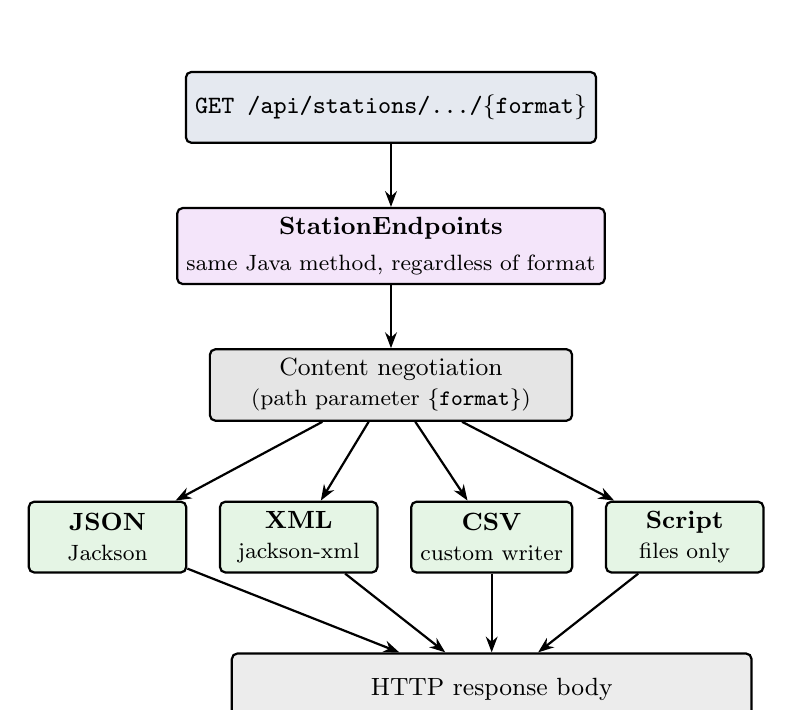
\begin{tikzpicture}[
      every node/.style={font=\small},
      box/.style={draw, rounded corners=2pt, align=center, thick,
                  minimum height=9mm, minimum width=22mm},
      writer/.style={box, fill=dkgreen!10, minimum width=20mm},
      arrow/.style={-{Stealth[length=2mm]}, thick}
    ]
    \node[box, fill=dkblue!10] (req) {\texttt{GET /api/stations/.../\{format\}}};
    \node[box, fill=mauve!10, below=8mm of req, minimum width=46mm]
      (resource) {\textbf{StationEndpoints}\\[2pt]\footnotesize same Java method, regardless of format};
    \node[box, below=8mm of resource, minimum width=46mm, fill=lgray]
      (negot) {Content negotiation \\\footnotesize (path parameter \texttt{\{format\}})};

    \node[writer, below=10mm of negot, xshift=-36mm] (json)   {\textbf{JSON} \\\footnotesize Jackson};
    \node[writer, right=4mm of json]                 (xml)    {\textbf{XML}  \\\footnotesize jackson-xml};
    \node[writer, right=4mm of xml]                  (csv)    {\textbf{CSV}  \\\footnotesize custom writer};
    \node[writer, right=4mm of csv]                  (script) {\textbf{Script}\\\footnotesize files only};

    \node[box, below=10mm of csv, fill=dark!10, minimum width=66mm]
      (resp) {HTTP response body};

    \draw[arrow] (req)       -- (resource);
    \draw[arrow] (resource)  -- (negot);
    \draw[arrow] (negot)     -- (json);
    \draw[arrow] (negot)     -- (xml);
    \draw[arrow] (negot)     -- (csv);
    \draw[arrow] (negot)     -- (script);
    \draw[arrow] (json)      -- (resp);
    \draw[arrow] (xml)       -- (resp);
    \draw[arrow] (csv)       -- (resp);
    \draw[arrow] (script)    -- (resp);
  \end{tikzpicture}%
  }
  \caption{Multi-format content negotiation in \texttt{api\_v4.0}. The
  same Java resource method is reused across four serializations,
  selected by a path parameter, and the differential harness must
  compare the body of each format separately.}
  \label{fig:multiformat}
\end{figure}

\subsection{\ac{JSON} and \ac{XML}}

\ac{JSON} is the default serialization and the format on which most
of the test fixtures of this project rely. The Jakarta \ac{REST}
implementation provided by Payara takes care of object serialization
through Jackson, with negligible per-request overhead. \ac{XML} is
provided by the \texttt{jackson-dataformat-xml} module, configured to
preserve the same Java models that produce \ac{JSON}. This dual
configuration is valuable because it removes a whole class of
\emph{schema drift} bugs: as long as the Java model is correct, both
\ac{JSON} and \ac{XML} outputs are consistent with each other.

\subsection{\ac{CSV}}

\ac{CSV} is the format favoured by historical clients of the \ac{API}
and is produced through a small set of writer classes that flatten
the entity tree into rows. The differential harness handles \ac{CSV}
exactly the same way it handles \ac{JSON} and \ac{XML}: the textual
body of the response is treated as an opaque blob that must match,
byte for byte, against the baseline.

\subsection{\ac{OpenAPI} and Swagger \ac{UI}}

The contract of the production \ac{API} is described in an
\ac{OpenAPI} 3.1.0~\cite{openapi} document
(\texttt{openapi.json}) that ships inside the \ac{WAR}. The same
document is served to a Swagger \ac{UI}~\cite{swaggerui} instance
hosted at \texttt{/swagger.html}, which provides an interactive,
in-browser playground for the endpoints. Two practical benefits arise
from this setup. First, the document is the single source of truth
shared with downstream consumers of the \ac{API}, in particular the
\ac{EPOS} portal. Second, the same document can be used to drive
contract tests: a future evolution of the test framework, briefly
discussed in Chapter~\ref{chap:conc-trab-futuro}, is to derive the
\ac{HTTP} differential test cases automatically from the \ac{OpenAPI}
specification instead of maintaining them in a separate \ac{JSON} file.

\section{Java and Jakarta EE}
\label{sec:java}

The applications target Java SE 21~\cite{javaSE21} (the production
\ac{API} and the second prototype) and Java SE 17 (the first
prototype, kept compatible with the \texttt{maven:\allowbreak 3.9.6-eclipse-\allowbreak temurin-21}
\ac{CI} image). The choice of Java was effectively imposed by the
existing code base; \texttt{record} types are used liberally for
request/response \acp{POJO} and the new \texttt{switch} expression
syntax replaces several long \texttt{if/else} chains from the legacy
\ac{API}.

\textbf{Jakarta EE 11}~\cite{jakartaee} provides the platform layer.
The renaming from Java EE in 2018 had already been absorbed by the
time this project started; the current code base targets the
\texttt{jakarta.*} package namespace. The specifications actively
used across the three applications are: Jakarta \ac{REST} 4.0
(\ac{JAX-RS})~\cite{jaxrs} for endpoints, Jakarta \ac{CDI} 4.1 for
injection, Jakarta Persistence 3.2 (\ac{JPA})~\cite{jpa} for
\ac{ORM}, Jakarta Bean Validation 3.1 for declarative constraints,
Jakarta JSON Binding 3.0 for serialization, and Eclipse
MicroProfile~\cite{microprofile} 2.1 \ac{JWT} (used by the second
prototype) plus Health 4.0 for probes. Spring Boot~\cite{springBoot}
was considered but rejected: the existing code base is already on
Jakarta EE on top of an existing Payara installation, and a parallel
migration would have brought no proportional benefit.

\section{\ac{SQL} and the Database Layer}
\label{sec:sql}

The persistence model of the production \ac{API} is heavily
relational: \ac{GNSS} stations, networks, agencies, countries, file
types, observation summaries and embargo windows are all linked
through foreign keys, and most endpoints execute several joins per
request. \ac{SQL}~\cite{postgresql} is therefore the natural query
language, and even where \ac{JPA}'s object-oriented abstractions
(Section~\ref{sec:jpa-hibernate}) are used, what reaches the database
is plain \ac{SQL}. The laboratory standardised on
\textbf{PostgreSQL}~\cite{postgresql} for the \ac{EPOS} production
database; the choice over \textbf{MySQL}~\cite{mysql} was driven
mainly by PostgreSQL's adherence to the \ac{SQL} standard (advanced
\texttt{JOIN} types, common table expressions, the
\texttt{numeric} type for high-precision station coordinates) and by
its rich set of index types (B-tree, BRIN, GiST). The PostGIS
extension is not in use today (Section~\ref{sec:epos-db}) but
remains a realistic future addition. MySQL was nevertheless used in
the docker-compose configuration of the second prototype
(Section~\ref{sec:prototypes}) to validate that the application-level
code is not tied to a specific dialect.

\subsection{\ac{JPA}, Hibernate and the Persistence Unit}
\label{sec:jpa-hibernate}

\ac{JPA}~\cite{jpa} is the Jakarta specification for object-relational
mapping in Java. The production \ac{API} uses
Hibernate~\cite{hibernate} as the \ac{JPA} provider, configured
through a \texttt{persistence.xml} file. The persistence unit is
named \texttt{MeuPU} and is declared as
\texttt{RESOURCE\_LOCAL}, which means that transactions are managed
explicitly by application code rather than by the container, a
deliberate choice that keeps the differential test harness in full
control of when transactions begin and end.

Database connections are pooled through \textbf{HikariCP}~\cite{hikaricp}
with a small, conservative pool (2--15 connections, 20-second connect
timeout, 30-second idle, 5-second validation), tuned for the
read-mostly workload of the \ac{API} and for the relatively low
concurrency observed in production.

\subsection{The \ac{EPOS} Database in Practice}
\label{sec:epos-db}

The production database lives on a PostgreSQL 16 instance reachable
from the laboratory network at \texttt{192.168.168.30:5432}, and the
same schema serves two fixtures: \texttt{DB\_3.0\_J}, a small but
representative production subset used by the correctness diffs, and
\texttt{DB\_3.0\_F}, the full dataset used for volume-oriented and
performance experiments. The schema contains forty-two tables and
around fifty foreign-key constraints, grouped into a core domain
(\texttt{station}, \texttt{network}, \texttt{agency},
\texttt{country}, \texttt{rinex\_file}, \texttt{highrate\_rinex\_file},
\texttt{file\_type}), the junction tables that materialise its
many-to-many relationships, a family of seven quality-control
summary tables, and a handful of auxiliary tables (embargoes,
documents, licenses, infrastructure). Station coordinates are
plain \texttt{numeric}; spatial logic is currently performed in Java
by the \texttt{Geometry} package rather than by PostGIS, which is
not installed (the only non-default extension is \texttt{plpgsql}).
The twenty-five existing indexes are mostly B-trees on foreign-key
columns, with \texttt{fillfactor=90} on the read-heavy quality-control
tables. The next planned optimisation, and the reason the larger
\texttt{F} fixture was provisioned, is the introduction of BRIN
indexes on the date columns of \texttt{rinex\_file}: \ac{RINEX} files
are written in approximate date order, so the on-disk layout already
correlates with the indexed column, which is the precondition for a
small and fast BRIN index. The differential framework introduced in
Chapter~\ref{chap:caso-epos} is used to validate that this
optimisation does not change observable behaviour against the
\texttt{F} fixture.

\section{Servers, Tooling and Network}
\label{sec:servers}

\textbf{Payara Server}~\cite{payara} is the Jakarta EE application
server adopted by the laboratory; the production \ac{API} is deployed
onto an existing Payara installation. Its companion product,
\textbf{Payara Micro}, is a single self-contained \ac{JAR} that
launches a deployable \ac{WAR} from the command line and is the
engine on which the \ac{HTTP}-level differential harness relies (the
harness boots one Payara Micro per \ac{WAR} on different ports and
replays the same requests against each). Apache Tomcat~\cite{apacheTomcat}
was considered for the prototypes but rejected because it does not
ship a full Jakarta EE 11 runtime out of the box.

All three applications are built with \textbf{Apache Maven}; the
production \texttt{pom.xml} configures, among others, the
\texttt{maven-war-plugin} (which produces the deployable
\texttt{ROOT.war}), \texttt{maven-failsafe-plugin} (integration tests
named \texttt{*IT.java} with \ac{JUnit} XML output) and
\texttt{maven-dependency-plugin} (which stages the Payara Micro
\ac{JAR} into \texttt{target/payara-micro/} so the \ac{HTTP} harness
can spawn it as a subprocess).

\textbf{GitLab}~\cite{gitlabci} provides both the source-control
front end and the \ac{CI}/\ac{CD} platform. The GitLab server is a
self-managed installation~\cite{gitlabSelfManaged} running on a
\ac{VM} inside the laboratory; the GitLab Runner~\cite{gitlabRunner}
is a separate process on another \ac{VM} (tagged
\texttt{ubi-runner-.31}) that picks up jobs and executes them inside
Docker containers. That separation matters because the runner is the
machine that needs network access to the laboratory's database, not
the control plane. \textbf{Git}~\cite{chacon2014pro} itself is used
non-trivially in the pipeline: \texttt{git worktree} is what
materialises each baseline build alongside the \texttt{HEAD} build on
the runner's filesystem, without disturbing the working copy
(Section~\ref{sec:pipeline}). All three repositories are hosted on
\texttt{gitlab.com}, the production \ac{API} under the
\texttt{segalubi} group, the two prototypes under the personal
namespace of the author.

\textbf{Docker}~\cite{docker} appears in two roles. \ac{CI} jobs run
inside the official
\texttt{maven:\allowbreak 3.9.6-eclipse-\allowbreak temurin-21} image,
which guarantees a clean and reproducible toolchain regardless of the
runner host. The two prototypes additionally ship a
\texttt{docker-compose.yaml}~\cite{composeSpec} for local development
(PostgreSQL plus, in the first prototype, a pair of Payara Server
containers for the dual-node Arquillian tests). The production
\ac{API} is intentionally \emph{not} containerised: the deployment
model is to copy the \ac{WAR} onto an existing Payara installation,
and an image would add a moving part with no benefit (this is
revisited in Chapter~\ref{chap:conc-trab-futuro}).

Finally, the production database is reachable only inside the
laboratory's network on \texttt{192.168.168.30:5432}, which is why
the runner is pinned by tag and why developers operating from outside
connect through the laboratory's \ac{VPN}, maintained by the SEGAL
staff. Alternatives such as WireGuard~\cite{wireguard} were
considered as lighter-weight options for one-off remote sessions but
were not adopted.

\section{Conclusion}
\label{chap3:sec:concs}

The technology stack on which this project is built is in large part
imposed by its environment: Jakarta EE on Payara, PostgreSQL on the
internal network, GitLab as the self-managed \ac{CI} platform. Where
there was room for choice, between Jakarta EE and Spring Boot,
between Payara Server and Apache Tomcat, between PostgreSQL and
MySQL, between JUnit 5 and TestNG, the decisions documented in
this chapter were guided by a preference for fewer moving parts, by
the alignment with what the laboratory already runs in production
and by the desire to keep the differential testing harness as simple
as possible. The next chapter describes the iterative methodology by
which these technologies were combined into a working solution.

\clearpage{\thispagestyle{empty}\cleardoublepage}
\chapter{Methodology and Architecture}
\label{chap:metodo-arq}

\section{The Legacy API}
\label{sec:legacy}

The starting point of the work is a code base that had grown organically for
several years and that nobody fully understood anymore: the previous
version of the \ac{EPOS} \ac{API} contained Java methods enormous scale, and
source files of an even larger scale, and many subtle behavioral quirks
introduced as patches by successive developers in response to specific bug
reports. Consequently, the laboratory could not confidently guarantee that
an arbitrary change would avoid silently breaking downstream \ac{API} clients.
While the full rewrite to Jakarta EE 11 significantly improved the internal
architecture introducing concise methods, cohesive \ac{JAX-RS} resources, and
a strict separation between parsing, validation, querying, and
serialization it also introduced a major regression risk. At any given commit
during the refactoring process, an endpoint might produce output subtly
different from the production baseline. The objective of this project is to construct
a testing harness that mitigates this risk, turning subtle data deviations
into immediate, actionable failures within the \ac{CI} pipeline.

\section{Iterative Methodology}
\label{sec:methodology}

The work was organized into three iterations, each carried out in its own
dedicated repository. This separation served two purposes. First, it kept each
iteration small and focused: the first prototype is deliberately stripped
down to two trivial endpoints, so that the entire complexity is in the \ac{CI}
configuration and not in the application; the second prototype is the opposite,
focusing on application code and leaving \ac{CI} aside; the production \ac{API}
then brings the two strands back together. Second, the prototypes have value
in their own right as didactic artifacts that future students of the laboratory
can read and re-use.

\section{Prototype Applications}
\label{sec:prototypes}

The first prototype, \texttt{java-ee-app}, validated the \ac{CI}/\ac{CD} infrastructure
end-to-end before any of the production code base was touched: it is a
minimal Maven \ac{WAR} exposing two trivial \ac{JAX-RS} endpoints, with a \texttt{.gitlab-ci.yml}
that builds the artifact and runs Arquillian integration tests against two
managed Payara Server containers declared as \emph{services} in the job.
Three patterns from that pipeline were carried over verbatim to the
production one: the pinned base image with the \texttt{ubi-runner} tag, the global
Maven repository cache, and the \texttt{reports: junit:} stanza that makes GitLab
understand assertion failures as failed pipeline steps.

The second prototype, \texttt{syncspace-jakarta-app}, focused on the
opposite concern: a complete Jakarta EE 11 application with no \ac{CI}
pipeline, exercising the specifications listed in Section~\ref{sec:java} on a
small room-booking domain (entities \texttt{User}, \texttt{Room}, \texttt{Booking})
protected by MicroProfile \ac{JWT}~\cite{microprofile}. \ac{JAX-RS}~\cite{jaxrs}
declares the resources, \ac{CDI} wires the services, \ac{JPA}~\cite{jpa} maps
the entities, Bean Validation enforces a custom \texttt{@ValidDateRange} constraint,
and a focused set of four \texttt{ExceptionMapper}s (\texttt{Business\-Validation\-Mapper},
\texttt{Validation\-Exception\-Mapper}, \texttt{Json\-Processing\-Exception\-Mapper},
\texttt{Global\-Exception\-Mapper}) translates domain and framework exceptions
into structured \ac{JSON} errors without leaking stack traces. The end-to-end
exception flow is summarised in Figure~\ref{fig:errormapper}.

\begin{figure}[H]
	\centering
	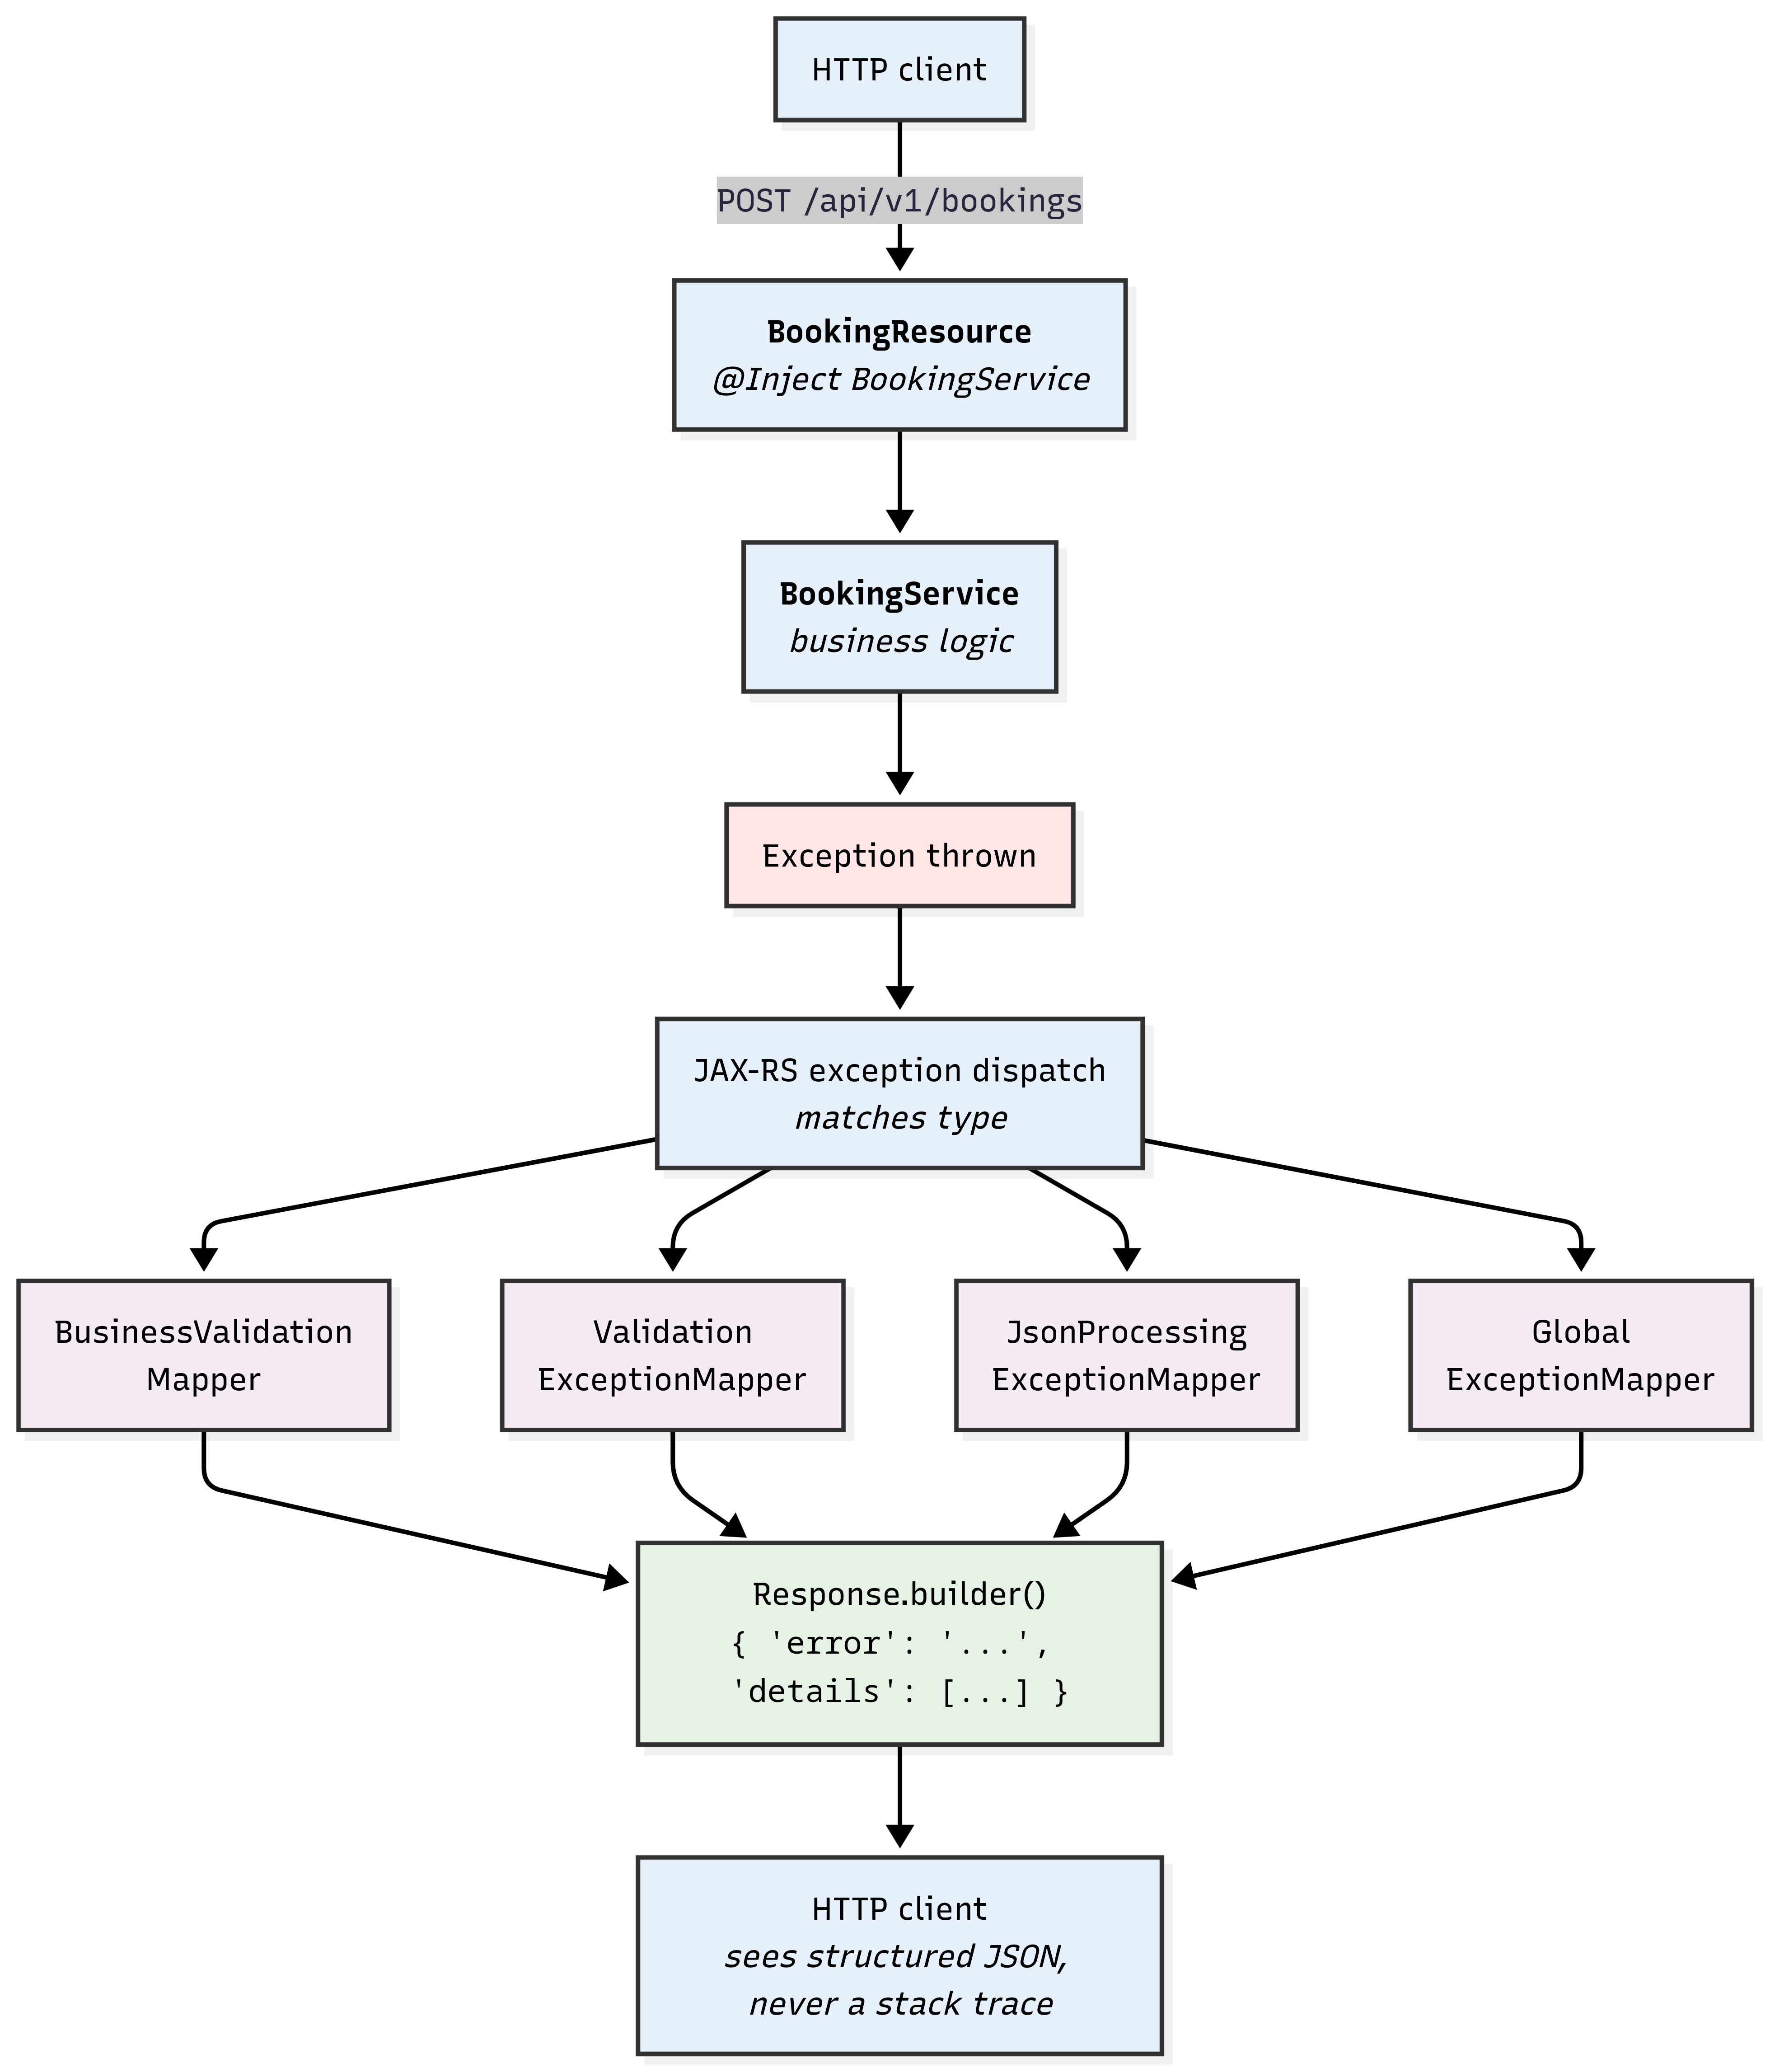
\includegraphics[width=\textwidth, height=14cm, keepaspectratio]{
		diagrams/syncspace-diagram.png
	}
	\caption{The \ac{CDI} + \ac{JAX-RS} exception-handling flow \ac{JSON} error
	body.}
	\label{fig:errormapper}
\end{figure}

Two patterns from \texttt{syncspace-jakarta-app} were adopted by the production
refactor: the use of a small set of focused \texttt{ExceptionMapper}s (which
keeps \ac{HTTP} status codes meaningful and gives the differential harness
a stable signal to assert on) and the use of \texttt{record}-based \acp{POJO}
for request and response bodies (which simplifies diffing). The remaining
features, in particular the full \ac{JWT} flow, were retained in the prototype
as a self-contained reference example for future students.

\section{Architecture of the Differential Testing Framework}
\label{sec:arch}

The architecture of the final testing framework, applied to the production \ac{API},
is summarised in Figure~\ref{fig:arch}. It is made of three concentric
layers: the GitLab pipeline, the harness processes, and the application instances
themselves.

\begin{figure}[H]
	\centering
	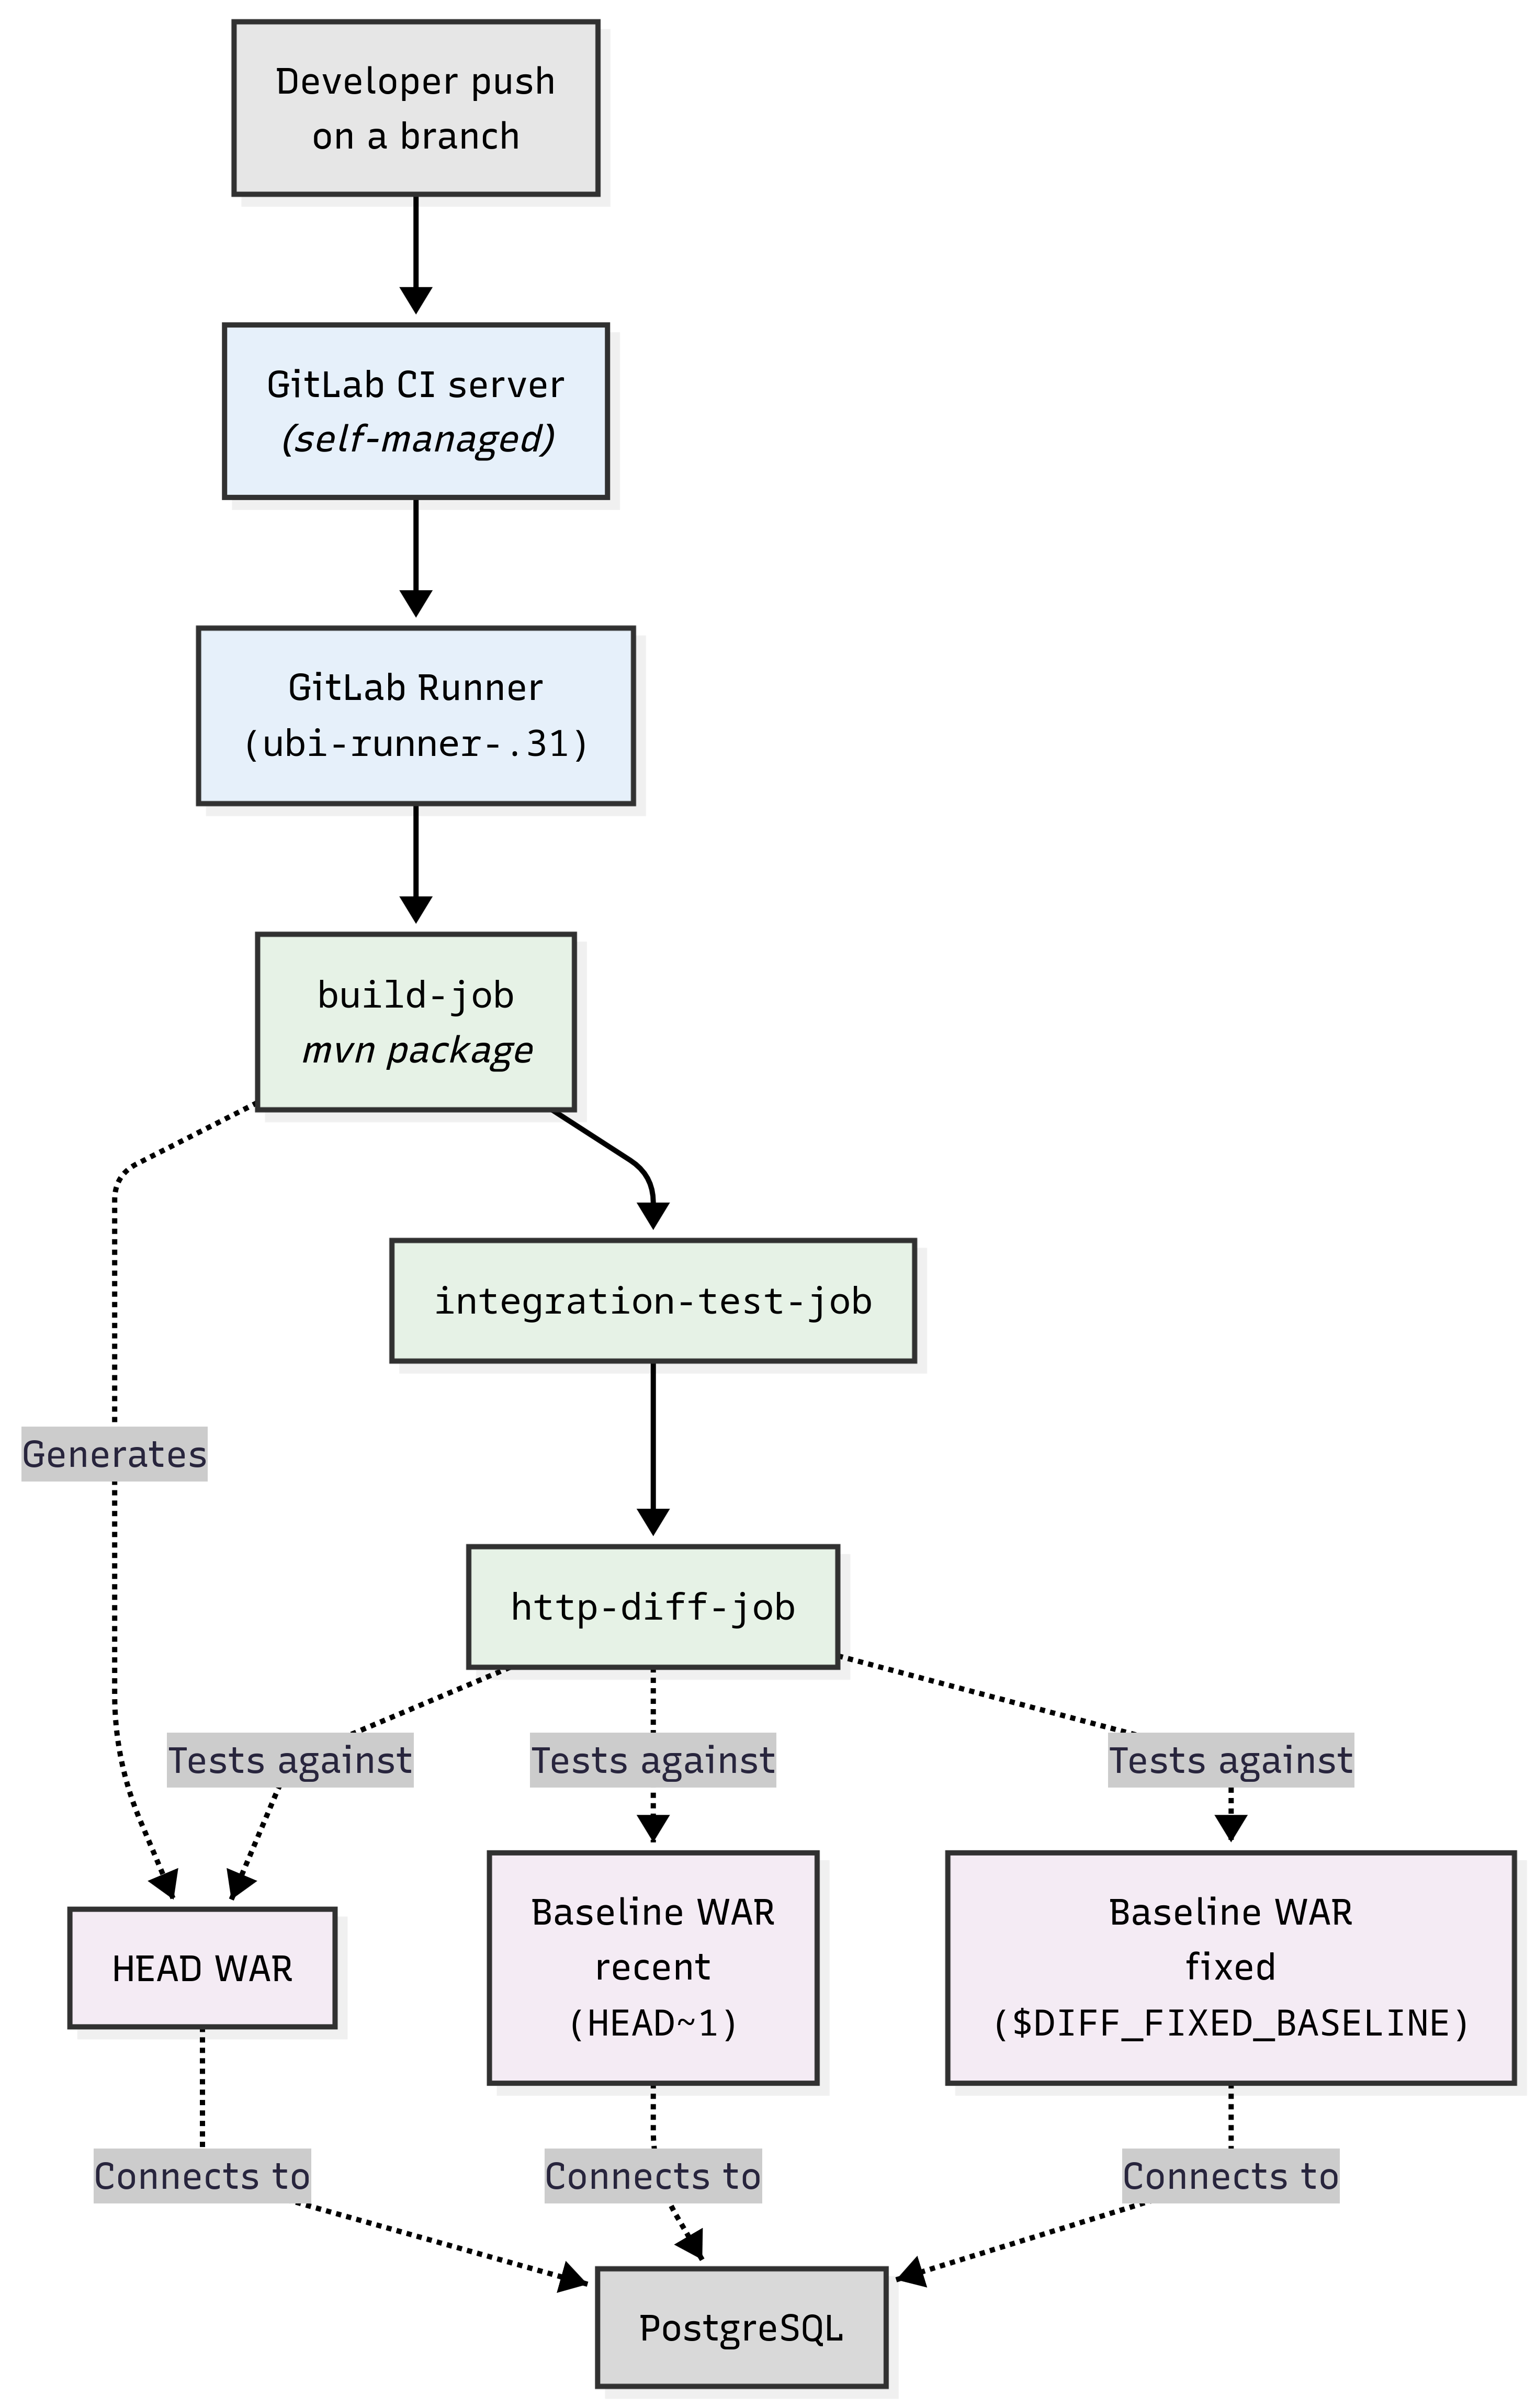
\includegraphics[width=\textwidth, height=14cm, keepaspectratio]{
		diagrams/ci-cd.png
	}
	\caption{Overall architecture of the differential testing framework.}
	\label{fig:arch}
\end{figure}

As illustrated, solid arrows denote execution flow, while dashed arrows
indicate artifact and data access. A developer push triggers a three-stage pipeline
on the internal runner (\texttt{ubi-runner-.31}):

First, \texttt{build-job} compiles the candidate \texttt{HEAD} \ac{WAR}. Second,
\texttt{integration-test-job} executes the standard JUnit suite. Finally, the
core \texttt{http-diff-job} performs a three-way comparison. It uses Git worktrees
to reconstruct both the immediate parent and a fixed reference baseline,
boots all three \acp{WAR} simultaneously on independent Payara Micro ports,
and replays \texttt{http-diff-cases.json} against a shared database fixture.
The resulting diff reports are then collected by GitLab as test artifacts.

Having refined this architecture through earlier prototypes---which traded
execution speed for a stricter separation of concerns---the next chapter
details the framework's application to the production \ac{API}.
\clearpage{\thispagestyle{empty}\cleardoublepage}
\chapter{Use Case: EPOS API}
\label{chap:caso-epos}

This chapter applies the framework of Chapter~\ref{chap:metodo-arq} to the
production \ac{API}, \texttt{api\_v4.0}. The \ac{EPOS} itself~\cite{epos} is
a pan-European research infrastructure in solid Earth science, organised
into Thematic Core Services for seismology, geomagnetic observations, \ac{GNSS}
data and products~\cite{eposGnss}, and so on; the \ac{SEGAL} laboratory of
\ac{UBI} contributes to the \ac{GNSS} service by operating a node that
hosts station metadata and \ac{RINEX}~\cite{rinex} observation files, and
\texttt{api\_v4.0} is the public interface of that node. Three properties
of the domain shape the test framework: the entities are relatively static (stable
baselines are easy to obtain), the typical client request returns a long
list of records (the comparison algorithm must scale to long diffs), and the
same information is exposed in several serialization formats (the surface
area to test multiplies but the underlying logic does not).

\section{Architecture of \texttt{api\_v4.0}}
\label{sec:apiv4-arch}

The application is a Maven \ac{WAR} project targeting Java SE 21 and Jakarta
EE 11, deployed onto Payara Server 6 with \texttt{finalName=ROOT} so that it
serves the root context. Its source tree is organised into four top-level
packages that form a classical layered architecture (Figure~\ref{fig:apiv4-layers}):
\texttt{Glass} provides the \ac{REST} layer (\ac{JAX-RS} resources \texttt{StationEndpoints},
\texttt{FilesEndpoints}, \texttt{ListEndpoints} and \texttt{Start}, plus
parsers, format writers and the validation/shape helpers); \texttt{Geometry}
and the helper classes \texttt{Validate.java} and \texttt{Shape.java} form
a thin business layer; \texttt{DB\_Tables} holds the forty \ac{JPA} entities
that model the relational schema (stations, networks, agencies, file types,
observation summaries, embargoes); and \texttt{Config} (\texttt{Loader.java})
is the cross-cutting concern that handles bootstrap.

Solid arrows denote ordinary call/data flow; dashed arrows denote
configuration and infrastructure binding established at deployment time.

\begin{figure}[h]
	\centering
	\resizebox{\linewidth}{!}{%
	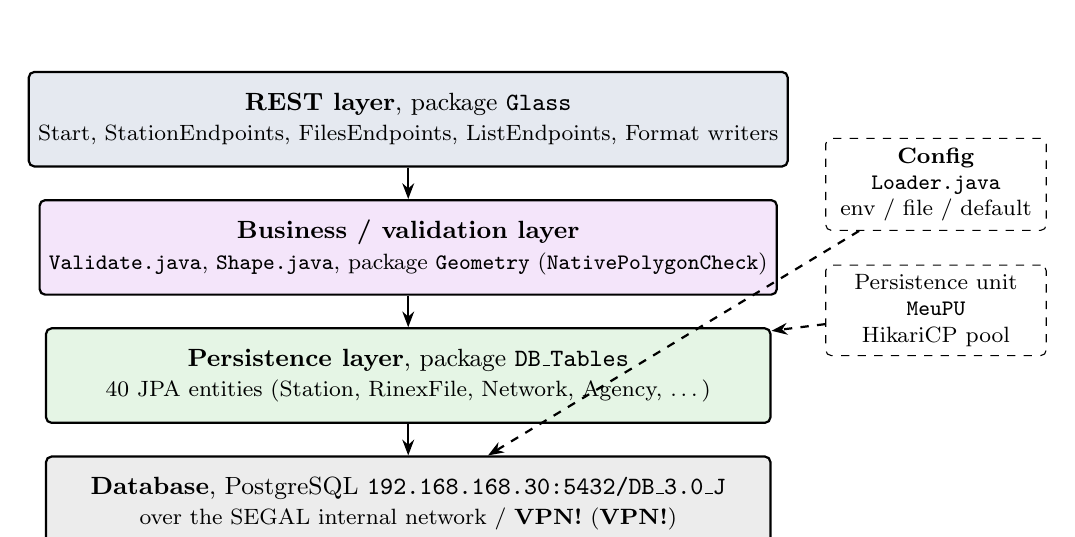
\begin{tikzpicture}[
		every node/.style={font=\small},
		node distance=4mm,
		layer/.style={draw, rounded corners=2pt, align=center, thick, minimum width=92mm, minimum height=12mm},
		cc/.style={draw, dashed, rounded corners=2pt, align=center, minimum width=28mm, minimum height=10mm, font=\footnotesize},
		arrow/.style={-{Stealth[length=2mm]}, thick}
	]
		\node[layer, fill=dkblue!10]
			(rest)
			{\textbf{REST layer}, package \texttt{Glass} \\ \footnotesize Start, StationEndpoints, FilesEndpoints, ListEndpoints, Format writers};
		\node[layer, fill=mauve!10, below=of rest]
			(biz)
			{\textbf{Business / validation layer} \\ \footnotesize \texttt{Validate.java}, \texttt{Shape.java}, package \texttt{Geometry} (\texttt{NativePolygonCheck})};
		\node[layer, fill=dkgreen!10, below=of biz]
			(jpa)
			{\textbf{Persistence layer}, package \texttt{DB\_Tables} \\ \footnotesize 40 JPA entities (Station, RinexFile, Network, Agency, \ldots)};
		\node[layer, fill=dark!10, below=of jpa]
			(db)
			{\textbf{Database}, PostgreSQL \texttt{192.168.168.30:5432/DB\_3.0\_J} \\ \footnotesize over the SEGAL internal network / \ac{VPN}};

		\node[cc, right=6mm of biz, yshift=8mm]
			(cfg)
			{\textbf{Config} \\\texttt{Loader.java} \\ env / file / default};
		\node[cc, right=6mm of biz, yshift=-8mm]
			(pu)
			{Persistence unit \\\texttt{MeuPU} \\ HikariCP pool};

		\draw[arrow] (rest) -- (biz);
		\draw[arrow] (biz) -- (jpa);
		\draw[arrow] (jpa) -- (db);
		\draw[arrow, dashed] (cfg) -- (db);
		\draw[arrow, dashed] (pu) -- (jpa);
	\end{tikzpicture}%
	}
	\caption{Layered architecture of \texttt{EPOS V4}.}
	\label{fig:apiv4-layers}
\end{figure}

\subsection{Endpoints and Output Formats}

The \ac{REST} surface is declared in four classes inside the \texttt{Glass}
package. \texttt{Start.java} carries the \texttt{@ApplicationPath("/api")} annotation
and registers a \texttt{PingResource} for the trivial \texttt{/api/ping} liveness
check. The three substantive resources are \texttt{StationEndpoints} (\texttt{/api/stations},
seven endpoints for station metadata indexed by identifier, location,
agency, network, equipment or coordinates), \texttt{FilesEndpoints} (\texttt{/api/files},
four endpoints for \ac{RINEX} file metadata filtered by agency/antenna/bounding
box/date, by marker, the high-rate variant, and an aggregated combination),
and \texttt{ListEndpoints} (\texttt{/api/list}, a parametric endpoint
returning the valid values of a given filter). Every endpoint accepts a
\texttt{\{format\}} path parameter and emits \ac{JSON}, \ac{XML}, \ac{CSV}
or (for the file endpoints) a downloadable shell script; the same \ac{OpenAPI}
3.1.0 document is served at \texttt{/swagger.html} through a Swagger \ac{UI}
hosted inside the \ac{WAR}.

\subsection{Persistence}

The persistence unit, declared in \texttt{src/\allowbreak main/\allowbreak
resources/\allowbreak META-INF/\allowbreak persistence.xml}, is named
\texttt{MeuPU} (inherited from the legacy code). It is configured as
\texttt{RESOURCE\_LOCAL}, with Hibernate as the \ac{JPA} provider and a connection
pool managed by HikariCP\@. Database connection parameters, host, port,
database name, user, password, are resolved at startup by \texttt{Config/Loader.java},
with the following precedence: environment variables, then a \texttt{Config.config}
file at the root of the deployment, then hard-coded defaults pointing at the
laboratory's database (\texttt{192.168.168.30:5432}).

The laboratory maintains two database fixtures with the same schema but
different volumes of data:

\begin{itemize}
	\item \texttt{DB\_3.0\_J} hosts a small but representative production
		subset, on the order of ten stations, eighty-six networks, two hundred and
		thirty agencies and roughly one hundred and forty-six thousand \texttt{rinex\_file}
		rows at the time of writing. This is the fixture used by the correctness
		diff runs, because it is small enough to allow per-case comparison of
		full response bodies without overwhelming the report.

	\item \texttt{DB\_3.0\_F} hosts the full dataset and is used by the
		volume-oriented diff runs, where the goal is not byte-for-byte equality but
		the detection of changes that would only be apparent at scale, for
		example, an inadvertent \texttt{N+1} query introduced by a refactor, or a
		query plan regression visible only on a large table.
\end{itemize}

The precedence rules of \texttt{Loader.java} are what allow the \texttt{http-diff-job}
to switch the running \acp{WAR} between the two fixtures without rebuilding
the artifact: the job sets the appropriate environment variables in its \texttt{variables:}
block and the application picks them up at boot.

The shape of the schema is discussed in Section~\ref{sec:epos-db}; a simplified
view of the central entities is given in Figure~\ref{fig:datamodel}.

Representative columns as they appear in the live PostgreSQL schema. Green
entities carry domain data; purple entities are controlled-vocabulary lookups
(note that \texttt{country.iso\_code} is the natural primary key, not a
surrogate \texttt{id}); grey entities are junction tables that materialise the
many-to-many relationships of the model. Arrows point from the ``one'' side
to the ``many'' side of the relationship.

\begin{figure}[h]
	\centering
	\resizebox{\linewidth}{!}{%
	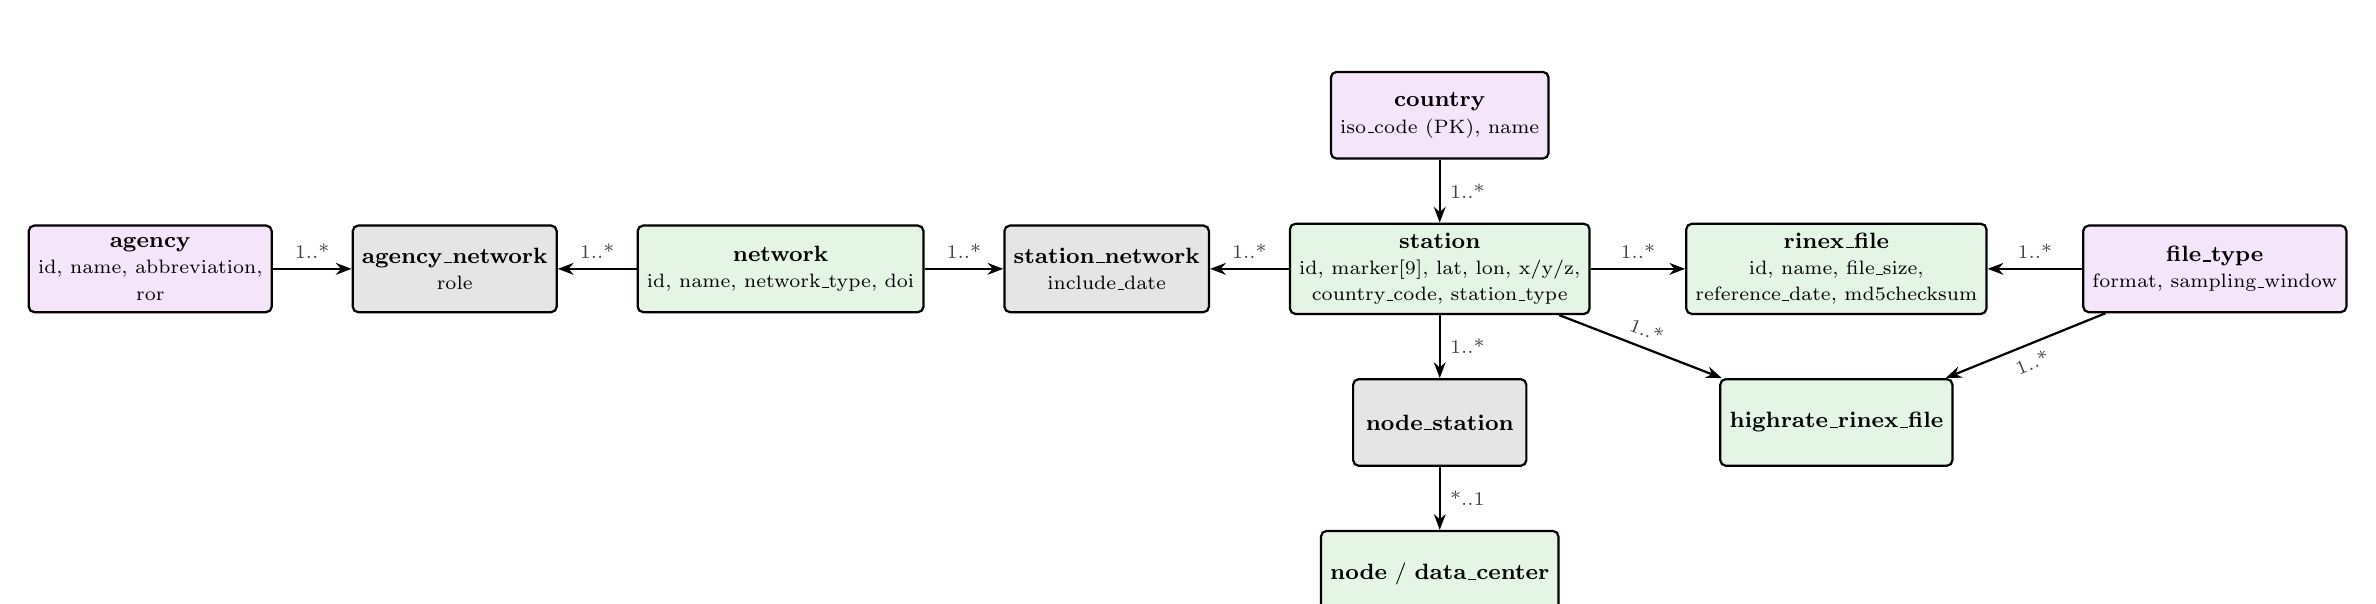
\begin{tikzpicture}[
		every node/.style={font=\footnotesize},
		entity/.style={draw, rounded corners=2pt, align=center, thick, minimum width=24mm, minimum height=11mm, fill=dkgreen!10},
		lookup/.style={entity, fill=mauve!10},
		junc/.style={entity, fill=lgray, minimum width=22mm},
		arrow/.style={-{Stealth[length=2mm]}, thick},
		rel/.style={font=\scriptsize, text=dark}
	]
		\node[entity]
			(station)
			{\textbf{station} \\\scriptsize id, marker[9], lat, lon, x/y/z,\\\scriptsize country\_code, station\_type};
		\node[junc, left=10mm of station]
			(sn)
			{\textbf{station\_network} \\\scriptsize include\_date};
		\node[entity, left=10mm of sn]
			(network)
			{\textbf{network} \\\scriptsize id, name, network\_type, doi};
		\node[junc, left=10mm of network]
			(an)
			{\textbf{agency\_network} \\\scriptsize role};
		\node[lookup, left=10mm of an]
			(agency)
			{\textbf{agency} \\\scriptsize id, name, abbreviation,\\\scriptsize ror};
		\node[lookup, above=8mm of station]
			(country)
			{\textbf{country} \\\scriptsize iso\_code (PK), name};
		\node[entity, right=12mm of station]
			(rinex)
			{\textbf{rinex\_file} \\\scriptsize id, name, file\_size,\\\scriptsize reference\_date, md5checksum};
		\node[entity, below=8mm of rinex]
			(highrate)
			{\textbf{highrate\_rinex\_file}};
		\node[lookup, right=12mm of rinex]
			(ftype)
			{\textbf{file\_type} \\\scriptsize format, sampling\_window};
		\node[junc, below=8mm of station] (nodest) {\textbf{node\_station}};
		\node[entity, below=8mm of nodest]
			(node)
			{\textbf{node} / \textbf{data\_center}};

		\draw[arrow] (agency) -- node[rel, above] {1..*} (an);
		\draw[arrow] (network) -- node[rel, above] {1..*} (an);
		\draw[arrow] (station) -- node[rel, above] {1..*} (sn);
		\draw[arrow] (network) -- node[rel, above] {1..*} (sn);
		\draw[arrow] (country) -- node[rel, right] {1..*} (station);
		\draw[arrow] (station) -- node[rel, above] {1..*} (rinex);
		\draw[arrow] (station) -- node[rel, above, sloped] {1..*} (highrate);
		\draw[arrow] (ftype) -- node[rel, above] {1..*} (rinex);
		\draw[arrow] (ftype) -- node[rel, below, sloped] {1..*} (highrate);
		\draw[arrow] (station) -- node[rel, right] {1..*} (nodest);
		\draw[arrow] (nodest) -- node[rel, right] {*..1} (node);
	\end{tikzpicture}%
	}
	\caption{Simplified view of the core \ac{EPOS} data model}
	\label{fig:datamodel}
\end{figure}

\section{The CI/CD Pipeline}
\label{sec:pipeline}

The pipeline of \texttt{api\_v4.0} extends the patterns validated on the first
prototype with an additional job in a new \texttt{diff} stage. The diff job compares
the current build against \emph{two} baselines, in what amounts to a three-way
comparison: the immediate parent commit \texttt{HEAD\textasciitilde 1} (which
catches regressions introduced by the commit currently being pushed) and a \emph{fixed}
reference commit identified by a SHA stored in the \texttt{DIFF\_FIXED\_BASELINE}
GitLab \ac{CI}/\ac{CD} variable (which catches the slow drift that
accumulates over many commits along a long-running refactor branch). The
key parts of the \texttt{.gitlab-ci.yml} are shown, condensed, in Listing~\ref{app:glass-ci-cd}.

Three details of the listing are worth highlighting. The \emph{recent} baseline
is \texttt{HEAD\textasciitilde 1}, which keeps the per-commit comparison focused
on the change just introduced; the \emph{fixed} baseline is a commit \ac{ID}
stored in \texttt{DIFF\_FIXED\_BASELINE} (typically pointing at the last
commit known to have shipped to the \ac{EPOS} portal) and acts as a long-term
reference against which the cumulative drift of the branch is measured. Each
baseline build is materialised through \texttt{git worktree} rather than
\texttt{git checkout}, so the working copy is never disturbed and the
harness can freely compare files from both checkouts in parallel. Finally,
each baseline is optional and treated independently: if \texttt{HEAD\textasciitilde
1} does not exist (first commit of the repository) or \texttt{DIFF\_FIXED\_BASELINE}
is unset (start of a refactor branch), the corresponding sub-run is skipped.
A pipeline can therefore have zero, one or two diff sub-runs depending on
the situation, and never fails because a baseline is simply unavailable.

\section{The HTTP-Level Diff: \texttt{HttpDiff.java}}
\label{sec:httpdiff}

\texttt{HttpDiff.java} is the harness that exercises the \ac{API} end-to-end.
Its execution proceeds in four phases, summarised graphically in Figure~\ref{fig:httpdiff-phases}.
The \ac{HTTP} harness runs once and internally boots \emph{all} the available
\acp{WAR} in parallel (the \texttt{HEAD} \ac{WAR}, the recent baseline if
any, and the fixed baseline if any). It then issues every test case against every
running instance and emits one diff report per baseline.

The harness boots one Payara Micro per available \ac{WAR}, the \texttt{HEAD}
build and whichever of the recent/fixed baselines were provided, waits for all
of them to be ready, fires every test case against every instance in
parallel, then performs a three-way comparison and emits one diff report per
baseline.

\begin{figure}[h]
	\centering
	\resizebox{\linewidth}{!}{%
	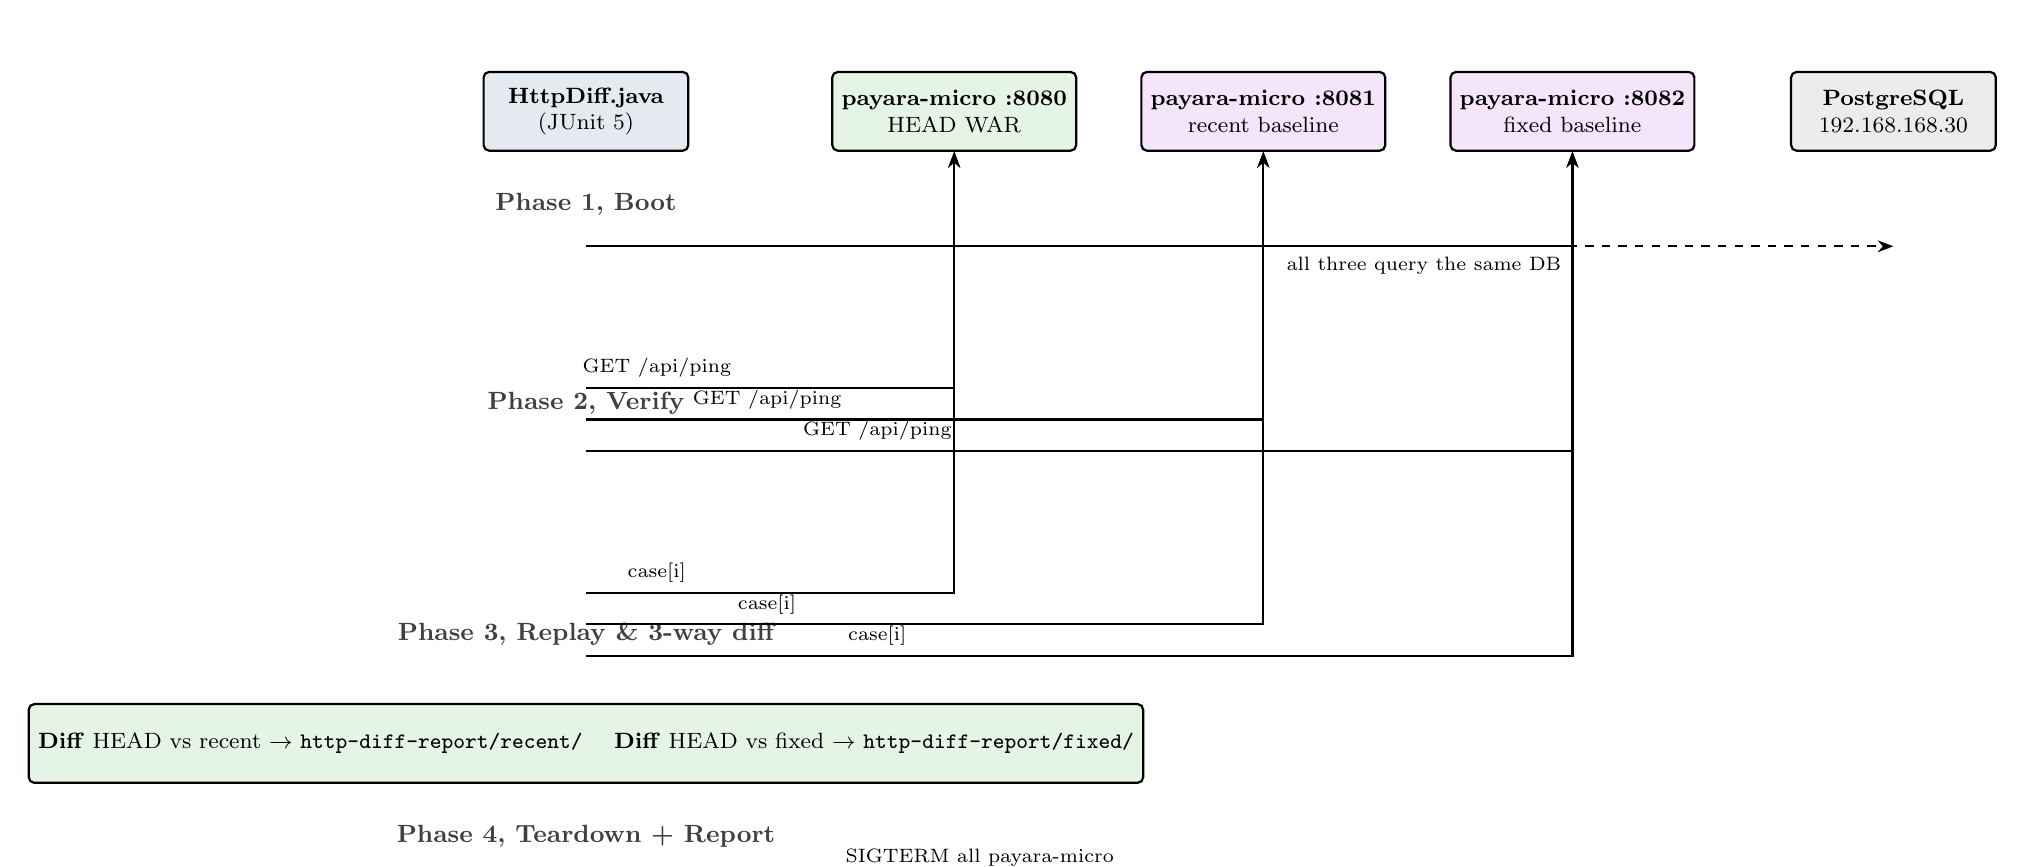
\begin{tikzpicture}[
		every node/.style={font=\footnotesize},
		proc/.style={draw, rounded corners=2pt, align=center, thick, minimum width=26mm, minimum height=10mm, fill=dkblue!10},
		micro/.style={proc, fill=mauve!10, minimum width=30mm},
		head/.style={proc, fill=dkgreen!10, minimum width=30mm},
		stage/.style={font=\small\bfseries, text=dark},
		barrow/.style={-{Stealth[length=2mm]}, thick},
		darrow/.style={-{Stealth[length=2mm]}, thick, dashed}
	]
		\node[proc]
			(harness)
			{\textbf{HttpDiff.java} \\ \footnotesize (JUnit 5)};
		\node[head, right=18mm of harness]
			(p80)
			{\textbf{payara-micro :8080} \\ \footnotesize HEAD WAR};
		\node[micro, right=8mm of p80]
			(p81)
			{\textbf{payara-micro :8081} \\ \footnotesize recent baseline};
		\node[micro, right=8mm of p81]
			(p82)
			{\textbf{payara-micro :8082} \\ \footnotesize fixed baseline};
		\node[proc, fill=dark!10, right=12mm of p82]
			(pg)
			{\textbf{PostgreSQL} \\ \footnotesize 192.168.168.30};

		\node[stage, below=4mm of harness] (s1) {Phase 1, Boot};
		\draw[barrow] ($(harness.south)+(0,-12mm)$) -| (p80.south);
		\draw[barrow] ($(harness.south)+(0,-12mm)$) -| (p81.south);
		\draw[barrow] ($(harness.south)+(0,-12mm)$) -| (p82.south);

		\node[stage, below=20mm of s1] (s2) {Phase 2, Verify};
		\draw[barrow]
			($(harness.south)+(0,-30mm)$) -- ++(1.8,0)
			node[midway, above, font=\scriptsize] {GET /api/ping}
			-|
			(p80);
		\draw[barrow]
			($(harness.south)+(0,-34mm)$) -- ++(4.6,0)
			node[midway, above, font=\scriptsize] {GET /api/ping}
			-|
			(p81);
		\draw[barrow]
			($(harness.south)+(0,-38mm)$) -- ++(7.4,0)
			node[midway, above, font=\scriptsize] {GET /api/ping}
			-|
			(p82);

		\node[stage, below=24mm of s2] (s3) {Phase 3, Replay \& 3-way diff};
		\draw[barrow]
			($(harness.south)+(0,-56mm)$) -- ++(1.8,0)
			node[midway, above, font=\scriptsize] {case[i]}
			-|
			(p80);
		\draw[barrow]
			($(harness.south)+(0,-60mm)$) -- ++(4.6,0)
			node[midway, above, font=\scriptsize] {case[i]}
			-|
			(p81);
		\draw[barrow]
			($(harness.south)+(0,-64mm)$) -- ++(7.4,0)
			node[midway, above, font=\scriptsize] {case[i]}
			-|
			(p82);
		\draw[darrow]
			($(p80.south)+(0,-12mm)$) -- ($(pg.south)+(0,-12mm)$)
			node[midway, below, font=\scriptsize] {all three query the same DB};

		\node[
			proc,
			fill=dkgreen!10,
			below=70mm of harness,
			minimum width=132mm
		]
			(diff)
			{\textbf{Diff} HEAD vs recent $\rightarrow$ \texttt{http-diff-report/recent/} \quad \textbf{Diff} HEAD vs fixed $\rightarrow$ \texttt{http-diff-report/fixed/}};

		\node[stage, below=4mm of diff] (s4) {Phase 4, Teardown + Report};
		\draw[barrow]
			($(harness.south)+(0,-92mm)$) -- ++(10.0,0)
			node[midway, above, font=\scriptsize] {SIGTERM all payara-micro};
	\end{tikzpicture}%
	}
	\caption{Phases of \texttt{HttpDiff.java}.}
	\label{fig:httpdiff-phases}
\end{figure}

The figure already covers the gist; a few implementation details are worth recording.
The test cases live in \texttt{src/\allowbreak test/\allowbreak resources/\allowbreak
http-diff-cases.json} as a \ac{JSON} array of request descriptors (method,
path, headers, optional body); This guards against spurious failures from
requests landing on still-deploying containers. Bodies are compared as normalised
strings (sorted \ac{JSON} keys, trimmed whitespace) and the headers that vary
by definition (\texttt{Date}, \texttt{Server}, \texttt{Content-Length}) are
ignored. The two comparisons (HEAD vs recent, HEAD vs fixed) are kept in
separate report directories so that a per-commit regression and an
accumulated drift remain distinguishable in the artifact tree.

\section{Reports and Findings}
\label{sec:reports}

Each pipeline run publishes the integration-test reports, the diff reports
(\texttt{recent/} and \texttt{fixed/} subdirectories of \texttt{target/http-diff-report/})
and the JUnit XML files consumed by GitLab. Integration test results expire
after one week; the diff reports are kept for four because they are the historical
record of behavioural change across the refactor. During development the
harness surfaced real regressions hidden inside seemingly cosmetic
refactors that no line-by-line review of the diff would plausibly have
caught by eye. The next chapter draws the main conclusions of the project and
outlines the items that, by choice or by constraint, were left out of its scope.
\clearpage{\thispagestyle{empty}\cleardoublepage}
\chapter{Conclusions and Future Work}
\label{chap:conc-trab-futuro}

\section{Main Conclusions}
\label{sec:conc-princ}

The work described in this report addresses a concrete problem of
the \ac{SEGAL} laboratory: how to refactor a large, several-years-old
Jakarta EE \ac{API} without silently breaking the \ac{EPOS} clients
that depend on it. The answer is a three-stage \ac{CI}/\ac{CD}-driven
testing framework that, for every commit, compares the new build
against two baselines (the immediate parent commit and a fixed
long-term reference) both at the level of internal Java classes and
at the level of \ac{HTTP} responses.

A few conclusions stand out. \emph{Differential testing fits a
refactor naturally}: asserting that the new build produces the same
output as a known-good one sidesteps the brittle fixture problem and
made the framework useful from the very first commit it ran on.
\emph{Two layers of comparison are better than one}: the code-level
harness catches behavioural changes in focused helper classes with
fast feedback, the \ac{HTTP}-level harness catches integration
regressions visible only against a live database, and neither one
alone covers the spectrum the laboratory cares about. \emph{A
self-hosted pipeline is not optional here}: only a runner inside the
laboratory's network can exercise the \ac{API} end-to-end against
the production database, so self-managing both the GitLab control
plane and the GitLab Runner host followed from the data-locality
constraint, not from a preference. \emph{The two prototypes paid for
themselves}: each answered a small, well-bounded set of questions in
an environment where mistakes were cheap, sparing the production
code base from them. \emph{The framework reveals what a human review
would miss}: the most representative example, discussed in
Section~\ref{sec:reports}, is the named-constants refactor of the
latitude/longitude bounds that no amount of code review would
plausibly have caught at the laboratory's commit rate.

\section{Future Work}
\label{sec:trab-futuro}

Several extensions to the framework were deliberately left out of
scope. The most immediate are the introduction of \textbf{BRIN}
indexes on the date columns of \texttt{rinex\_file} (and the
companion \emph{performance-regression subsystem} that would record
wall-clock durations against the \texttt{F} fixture to justify them
empirically), the \textbf{PostGIS migration} of the spatial helpers
in the \texttt{Geometry} package (with the same differential
framework used to verify byte-for-byte equivalence), and the
\textbf{automatic generation of \ac{HTTP} test cases} from the
\ac{OpenAPI} document shipped inside the \ac{WAR} (so newly added
endpoints are exercised by the diff from the moment they are
merged). The framework would also benefit from a \textbf{schema diff}
of the \ac{OpenAPI} document itself across builds (to surface
contract regressions distinct from behavioural ones), from a
\textbf{snapshot test} layer for endpoints that should remain stable
across releases (such as \texttt{/api/ping}), and from
\textbf{containerization of the production deployment} to remove
the residual gap between the \ac{WAR} that was tested and the
\ac{WAR} that ships. Finally, the harness code itself could be
\textbf{generalised into a small library} reusable by other Jakarta
EE services of the laboratory, with the application-specific bits
factored into a clean configuration interface; orthogonal to that,
several \textbf{operational aspects} (transient-error retries, clean
termination of orphan Payara Micro processes, automated provisioning
of the runner host, a long-term dashboard on top of the diff
reports) deserve more attention than the present project could
afford.

\bigskip

Overall, the framework delivered by this project addresses the
problem that motivated it, has already proved its value on a real
regression caught during the refactor, and lays the groundwork for
the laboratory to continue evolving the \ac{API} with a much higher
degree of confidence than was previously possible. The items listed
in this section are natural next steps; none of them invalidates
the design that was put in place.

\clearpage{\thispagestyle{empty}\cleardoublepage}

% Uncomment if appendices are added.
\appendix
% Just like a normal chapter file, you just start writing.
% Because the main file already threw the \appendix switch, 
% this \chapter will automatically become "Appendix A".

\chapter{Raw Survey Data}

Here is the table containing all 500 responses...
\clearpage{\pagestyle{empty}\cleardoublepage}

\backmatter

\bibliographystyle{unsrt}
\bibliography{bibliografia}

\end{document}
